\documentclass[11pt,twoside]{book}
\usepackage[spanish]{babel}
\usepackage{natbib}
\usepackage{url}

% referencias coma na pagina anterior, etc
\usepackage{bookman}
\usepackage[spanish]{varioref}
% acentuaci�n
\usepackage[latin1]{inputenc}
\usepackage{indentfirst}
\usepackage{ upgreek }
\usepackage{xspace}
\usepackage{url}
\usepackage{setspace}
\usepackage{graphicx}
\usepackage{fancybox}
\usepackage{amsmath}
\usepackage{amsfonts}
%\usepackage[bbgreekl]{mathbbol}
\usepackage{amssymb}
\usepackage{multirow}
\usepackage{booktabs}
\usepackage{paralist}
\usepackage{color}
\usepackage{subfigure}
\usepackage{amsmath}

\definecolor{red}{rgb}{0.9,0.1,0.1}
\definecolor{blue}{rgb}{0,0.1,0.8}

\usepackage[pdftex, plainpages=false, hyperfootnotes=false]{hyperref}
\hypersetup{colorlinks=true, linkcolor=blue, citecolor=blue, urlcolor=blue}
%%% bibliografia
\usepackage[sf,outermarks,clearempty]{titlesec}

\usepackage[pdftex]{geometry}
%m�rgenes del papel 
\geometry{a4paper,left=3cm,right=3cm,top=3cm,bottom=3cm,twoside}
%\geometry{a4paper,left=3cm,right=3cm,top=3cm,bottom=3cm,twoside}


\usepackage{acronym}

\usepackage[ruled,vlined,portugues,algochapter]{algorithm/algorithm2e}
\usepackage{algorithm/algorithmic-pt}  % Algoritmos em Portugues
\usepackage{eqparbox,array}
\renewcommand\algorithmiccomment[1]{%
    {// \small{\textit{#1}}}%
}
\newcommand\LONGCOMMENT[1]{%
  \hfill\#\ \begin{minipage}[t]{\eqboxwidth{COMMENT}}#1\strut\end{minipage}%
}

\acrodef{CBIR} {Content-based Image Retrieval}
\acrodef{MAM}  {M�todos de Acceso M�trico}
\acrodef{SAM}  {M�todos de Acceso Espacial}
\acrodef{MAE}  {M�todos de Acesso Espaciais}

\acrodef{DTW}  {Dynamic Time Warping}
\acrodef{LSH}  {Locality Sensitive Hashing}

\newtheorem{defi}{{\it Definici�n}}[chapter]
\newcommand{ \Correction }[ 1 ] {\textcolor{black}{#1}}
\newcommand{ \NewMaterial }[ 1 ] {\textcolor{black}{#1}}
\newcommand{ \ConnectDots }[ 1 ] {\textcolor{black}{#1}}
\newcommand{ \NewMaterialGPU }[ 1 ] {\textcolor{green}{#1}}
\newcommand{ \Error }[ 1 ] {\textcolor{red}{#1}}

% Different font in captions
\newcommand{\captionfonts}{\small}

%defina o tamanho da barra na tabela de cronograma
\newcommand{\barrai}[1]{\rule{#1}{2mm}}
\newcommand{\barrad}[2]{\hspace{#1} \rule{#2}{2mm}}

% declara 'e' para fun��o exponencial
\DeclareMathOperator{\e}{e}

\makeatletter  % Allow the use of @ in command names
\long\def\@makecaption#1#2{%
  \vskip\abovecaptionskip
  \sbox\@tempboxa{{\captionfonts #1: #2}}%
  \ifdim \wd\@tempboxa >\hsize
    {\captionfonts #1: #2\par}
  \else
    \hbox to\hsize{\hfil\box\@tempboxa\hfil}%
  \fi
  \vskip\belowcaptionskip}
\makeatother   % Cancel the effect of \makeatletter

%fonte
%\usepackage{ae}
%\usepackage[T1]{fontenc}
%\DeclareFixedFont{\numberfont}{T1}{phv}{bx}{n}{2cm}

%%% redefine o formato do t�tulo
\titleformat{\chapter}[display]
  {\normalfont\Large\sffamily
  }
  {%\titlerule[3pt]%
   \filright
   \rule[32pt]{.7\linewidth}{4pt}
   \hspace{-11pt}
   \shadowbox{
   \begin{minipage}{.18\linewidth}
     \begin{center}
       \textsc{\Large\chaptertitlename}\\
       \vspace{1ex}
       { \thechapter}\\
       \vspace{1ex}
     \end{center}
   \end{minipage}}
  }
  {0pt}
  {\filcenter
   \Huge
   }
  [\hfill\rule{.8\textwidth}{0.5pt}\\
     \vskip-1.8ex\hfill\rule{.7\textwidth}{3pt}]


% primeira letra do texto
\font\largefont = pzcmi7t scaled 6500
\newcommand{\versal}[1]{{\noindent
    \setbox0\hbox{\largefont #1 }%
    \count0=\ht0                   % height of versal
    \count1=\baselineskip          % baselineskip
    \divide\count0 by \count1      % versal height/baselineskip
    \dimen1 = \count0\baselineskip % distance to drop versal
    \advance\count0 by 1\relax     % no of indented lines
    \dimen0=\wd0                   % width of versal
    \global\hangindent\dimen0      % set indentation distance
    \global\hangafter-\count0      % set no of indented lines
    \hskip-\dimen0\setbox0\hbox to\dimen0{\raise-\dimen1\box0\hss}%
    \dp0=0in\ht0=0in\box0}}


%-------------PARA CITAR PAGINAS--------------------


%\hyphenpenalty=2000
%\tolerance=2000
\hyphenpenalty=5000
\tolerance=5000


\hyphenation{di-men-sio-na-li-da-de}
\hyphenation{uni-di-men-sional}
\hyphenation{multi-di-men-sional}
\hyphenation{re-pre-sen-ta-coes}

%aqu� comienza el documento.

\begin{document}
\begin{titlepage}
\pagestyle{empty}

%\begin{flushright}
%\begin{Sbox}
%\begin{minipage}{8.5cm}
%\footnotesize
%UNIVERSIDAD NACIONAL DE SAN AGUST�N\\
%\\
%Fecha de Registro: 31/08/2015\\
%\\
%Asignatura:\hrulefill
%\end{minipage}
%\end{Sbox}
%\fbox{\TheSbox}
%\end{flushright}

\vspace*{3cm}
\begin{center}
{\Large\sf Visualizaci�n de la evoluci�n temporal de datos multidimensionales usando �rboles filogen�ticos enfocado en art�culos cient�ficos}

% visualizaci�n temporal
% evoluci�n temporal de temas / temporal evolution of topics
% proyeccion de datos multidimensionales 
% colecciones de art�culos cient�ficos
% �rboles filogen�ticos 

\vspace*{2cm}

{\it Roberto Josu� Rodr�guez Urquiaga}

\vspace*{1.5cm}

{\bf Asesor:}  {\it Dra. Ana Maria Cuadros Valdivia}

\vspace*{0.5cm}


\end{center}

\vspace*{3.5cm}

\begin{flushright}
\begin{minipage}{10cm}
Tesis presentada a la Universidad Nacional de San Agust�n como parte de los requisitos para obtener el grado acad�mico de Maestro en Inform�tica con Menci�n en Tecnolog�as de Informaci�n.
\end{minipage}
\end{flushright}

\vspace*{2.5cm}
\begin{center}
\textbf{UNSA - Arequipa \\ Agosto - 2016}
\end{center}
%\cleardoublepage



\vfill

\vspace*{5cm}

\begin{center}
\begin{minipage}[c]{12cm}
\begin{center}
\hrulefill\\
\vspace{.5cm} {\Large Visualizaci�n de la evoluci�n temporal de datos multidimensionales usando �rboles filogen�ticos enfocado en art�culos cient�ficos}\\
\vspace{1.3cm}
\textbf{\it Roberto Josu� Rodr�guez Urquiaga}\\
\vspace{.5cm}
\hrulefill\\
\end{center}
\end{minipage}
\end{center}

\vfill

%\cleardoublepage

\end{titlepage}


\pagenumbering{roman}


\chapter*{Resumen}

\addcontentsline{toc}{section}{Resumen}

En la actualidad la cantidad de datos producida por los medios electr�nicos a tenido un alza importante tanto en n�mero de registros como en complejidad, como consecuencia identificar informaci�n �til de estos grandes conjuntos de datos se ha vuelto un reto, una gran parte de esta aumento en la cantidad de datos viene relacionado a las colecciones de art�culos cient�ficos que recientemente su exploraci�n a despertado el inter�s de la comunidad cient�fica, como consecuencia se han realizado trabajos para facilitar el an�lisis de estas colecciones de documentos usando t�cnicas de miner�a de datos y visualizaci�n de informaci�n, dentro de las t�cnicas de visualizaci�n de datos multidimensionales se encuentran las \textit{Proyecci�n multidimensional} que permiten reducir de una dimensiolidad alta a un espacio de dimensi�n ya sea $1, 2, 3$ conservando las caracter�sticas de similitud de los datos en la dimensi�n original haciendo posible encontrar patrones a trav�s de la capacidad visual humana. La mayor�a de enfoques de proyecciones multidimensional de datos no considera el componente temporal de las colecciones de art�culos cient�ficos a pesar de tener el componente temporal un papel crucial en muchos tipos de datos, en este trabajo se propone incorporar el tratamiento del componente temporal en una proyecci�n multidimensional basado en �rboles filogen�ticos de modo que sea apropiado para tareas de an�lisis exploratoria envolviendo la evoluci�n de temas en colecciones de art�culos cient�ficos.


 
\singlespacing
\vspace*{0.5cm} \noindent \textbf{Palabras Clave:} 
Visualizaci�n temporal de documentos, evoluci�n temporal de temas, �rboles filogen�ticos, proyecci�n de datos multidimensionales.
\chapter*{Abstract}

\addcontentsline{toc}{section}{Abstract}
Currently the amount of data produced by the electronic media had a significant increase in number of records and complexity, as a result identify useful information from these large data sets has become a challenge, a large part of this increase in the amount of data is related to collections of scientific papers recently its exploration aroused the interest of the scientific community, following work has been done to facilitate analysis of these collections of documents using techniques of data mining and information visualization within visualization techniques multidimensional data are the \ textit {multidimensional projection} that reduce a high dimensiolidad to a space dimension either $ 1, 2, 3 $ preserving the characteristics of similarity of the data in the dimension Original making it possible to find patterns through the human visual capacity. Most approaches to multidimensional data projections does not consider the temporal component of the collections of scientific papers despite having the time component a crucial role in many types of data, this paper intends to incorporate the treatment of temporal component in a projection multidimensional based on phylogenetic trees so that it is appropriate for exploratory analysis tasks involving the evolution of issues in collections of scientific articles.

\singlespacing
\vspace*{0.5cm} \noindent \textbf{Keywords:}  Temporal visualization of documents, temporal evolution of topics, phylogenetic trees, multidimensional data projection


%\cleardoublepage

\addcontentsline{toc}{section}{Sumario}
\tableofcontents

%\cleardoublepage
%----------- lista de s�mbolos ----------------
%\addcontentsline{toc}{section}{Lista de S�mbolos}
%\chapter*{Lista de S�mbolos}

%\setstretch{1.25}
%\begin{tabular}{ l l l l }
    %$\mathbb{S}$ & universo %de datos\\
%\end{tabular}
%\cleardoublepage
%\singlespacing

%------- agregamos la lista de todos los elementos --

\listoffigures
\addcontentsline{toc}{section}{Lista de Figuras}
\cleardoublepage
\listoftables
\addcontentsline{toc}{section}{Lista de Tablas}
\cleardoublepage

%\listofalgorithms
%\addcontentsline{toc}{section}{Lista de Algoritmos}
%\cleardoublepage

\pagestyle{plain}
\onehalfspace
\pagenumbering{arabic}
%agregando los archivos
\chapter{Introducci�n}

\section{Consideraciones Iniciales}\label{sec:in}
%\versal{E}
%\versal{E}n el campo de la investigaci�n en general, los art�culos cient�ficos son el mejor mecanismo por medio del cual los investigadores publican sus resultados \citep{147:alencar:2012}. Son muy importantes al momento de iniciar una nueva investigaci�n, debido a que se requiere de una b�squeda y revisi�n de los trabajos m�s cercanos al tema de investigaci�n \citep{154:sun:2013}. Actualmente las bases de datos cient�ficas permiten realizar esta labor y para buscar art�culos cient�ficos en estos sistemas inform�ticos generalmente se emplean interfaces tradicionales, compuestas por formularios, ventanas, men�s, etc. Adem�s se utilizan palabras claves, el nombre del autor, el a�o de publicaci�n como par�metros de b�squeda y se presentan los resultados generalmente como una lista textual \citep{153:sakai:2012}. Pero a medida que la informaci�n crece con celeridad, se presentan dificultades para explorar y seleccionar adecuadamente los art�culos cient�ficos en este tipo de interfaces tradiciones, que puede ocasionar que el investigador no encuentre la informaci�n deseada. Por tanto, es importante investigar nuevas formas de representar e interactuar con la informaci�n.

% la creciente alza de datos en internet
En la actualidad la cantidad de datos producida por los medios electr�nicos a tenido un alza importante tanto en el n�mero de registros como en complejidad, este exceso de informaci�n es conocido como "sobrecarga de informaci�n" y esto ocurre cuando una persona no es capaz de localizar o hacer uso de informaci�n que necesita \citep{christian2001information}, como consecuencia identificar informaci�n �til de estos grandes conjuntos de datos se ha vuelto un reto, pues si ning�n tipo de informaci�n es extra�da el almacenamiento de los mismos sera una tarea in�til \citep{keim2002information}.
% los articulos cientificos
Una gran parte de esta aumento en la cantidad de datos viene relacionado a las colecciones de art�culos cient�ficos que recientemente su exploraci�n a despertado el inter�s de la comunidad cient�fica, pues son muy importantes al momento de iniciar una nueva investigaci�n \citep{154:sun:2013}, a pesar que los motores de bases de datos cient�ficas ayudan en esta labor sus resultados son mostrados en una lista textual \citep{153:sakai:2012} y esto crea un problema cuando se van creando con el tiempo nuevas investigaciones ocasionando dificultados en el proceso de exploraci�n por parte de un investigador. Como consecuencia se han realizado trabajos para facilitar el an�lisis de estas colecciones de documentos como por ejemplo en los trabajos de \citep{paulovich2008least} , \citep{alencarvisualizaccao}, \citep{valdivia2007mapeamento}.

% tecnicas para analizar los arituclos cientificos


% evolucion temporal de los temas 
Los enfoques antes considerados ofrecen una visualizaci�n de los datos en este caso colecciones de art�culos cient�ficos, donde las similitudes de documentos es por contenido, y tienen la desventaja de no ofrecer una evoluci�n de sus temas a trav�s del tiempo, por ejemplo si un investigador quiere saber que cuales son las investigaciones mas recientes en un campo de estudio, las t�cnicas antes mencionadas no proporcionaran ayuda, para esto se ha realizado un enfoque en \citep{alencar2007mineraccao} donde aborda este problema haciendo uso tambi�n de t�cnicas conocidas como \textit{Temporal text mining} y \textit{Evolutionary theme patterns} \citep{mei2005discovering} enfoc�ndose principalmente en hacer una versi�n temporal de \textit{Least square projection}, el estudio antes mencionado permite visualizar patrones en las colecciones de art�culos dando una idea de su evoluci�n tem�tica temporal, aun as� tiene la desventaja de que la interpretaci�n de la visualizaci�n es dif�cil y necesita ser evaluada por un experto.

% NJ


\section{Motivaci�n}\label{sec:motivacion}
Las t�cnicas de proyecci�n han demostrado tener un buen desempe�o en cuanto a la visualizaci�n de informaci�n de varios tipos de datos incluyendo colecciones de art�culos cient�ficos \citep{valdivia2007mapeamento}, \citep{paulovich2008mapeamento}, sin embargo si se considera una colecci�n de art�culos cient�ficos que tienen propiedades temporales como es en el mayor numero de casos como una conferencia anual que a sido indexada temporalmente. A pesar de tener el componente temporal un papel crucial en muchos tipos de datos, inclusive en texto, muchas t�cnicas de proyecci�n multidimensional no lo consideran expl�citamente en su proceso de visualizaci�n \citep{alencarvisualizaccao}, algunos avances en esta �rea son las proyecciones din�micas como \textit{Temporal Least square projection} en \citep{alencarvisualizaccao} donde ofrece un enfoque temporal aplicado a un m�todo de proyecci�n, algunas deficiencias de este enfoque son la dificultad de analizar los resultados, en el trabajo antes mencionado tambi�n emplea t�cnicas como \textit{Temporal text mining} y \textit{Evolutionary theme patterns} para ver la evoluci�n temporal de temas, aun as� al algoritmo  \textit{Least square projection} tiene problemas para dar una correcta visualizaci�n de los mismos.

\section{Objetivos}\label{sec:objetivos}

\subsection{Objetivo Principal}
Investigar como incorporar el tratamiento del componente temporal en una proyecci�n multidimensional basado en �rboles filogen�ticos de modo que sea apropiado para tareas de an�lisis exploratoria envolviendo la evoluci�n de temas en colecciones de art�culos cient�ficos.

\subsection{Objetivos Secundario}
\begin{enumerate}
	\item Obtener una proyecci�n multidimensional con componente temporal basado en �rboles filogen�ticos.
	\item Detectar e incluir una representaci�n visual sobre la evoluci�n de t�picos o temas.
\end{enumerate}

\section{Organizaci�n del Trabajo} \label{sec:estrutura}

Este trabajo est� organizado en 5 cap�tulos, incluyendo esta introducci�n, y la siguiente estructura:

\begin{itemize}
 % similarity search
 
\item En el \textbf{Cap�tulo 2} se presenta los conceptos previos de la investigaci�n, el cual incluye Mineria de datos temporales, Evoluci�n temporal de temas, Proyecci�n de datos multidimensionales y �rboles filogen�ticos.

%\item En el \textbf{Cap�tulo 3} se describen todo el proceso de desarrollo de la investigaci�n, que implica el desarrollo de cada objetivo espec�fico a fin de alcanzar el objetivo general.

%\item En el \textbf{Cap�tulo 4} se muestra la evaluaci�n de los resultados, desde su representaci�n y an�lisis estad�stico hasta su interpretaci�n. Adem�s se presentan las publicaciones cient�ficas aceptadas, en evaluaci�n y en proceso de elaboraci�n.

%\item En el \textbf{Cap�tulo 5} se presentan las conclusiones finales de la investigaci�n, las contribuciones y los trabajos futuros.
\section{Descripci�n del problema}
 Identificar informaci�n �til de grandes conjuntos de datos se ha vuelto un reto \citep{keim2002information}, una gran parte de esta aumento en la cantidad de datos viene relacionado a las colecciones de art�culos cient�ficos que recientemente su exploraci�n a despertado el inter�s de la comunidad cient�fica, pues son muy importantes al momento de iniciar una nueva investigaci�n \citep{154:sun:2013}, a pesar que los motores de bases de datos cient�ficas ayudan en esta labor sus resultados son mostrados en una lista textual \citep{153:sakai:2012} y esto crea un problema cuando se van creando con el tiempo nuevas investigaciones ocasionando dificultados en el proceso de exploraci�n por parte de un investigador. Como consecuencia se han realizado trabajos para facilitar el an�lisis de estas colecciones de documentos como por ejemplo en los trabajos de \citep{paulovich2008least} haciendo uso del m�todo de proyecci�n  \textit{Least square projection} como en \citep{valdivia2007mapeamento} utiliza \textit{Neighbor joining}.
Los enfoques antes considerados ofrecen una visualizaci�n de los datos en este caso colecciones de art�culos cient�ficos, donde las similitudes de documentos es por contenido, y tienen la desventaja de no ofrecer una evoluci�n de sus temas a trav�s del tiempo, por ejemplo si un investigador quiere saber que cuales son las investigaciones mas recientes en un campo de estudio, las t�cnicas antes mencionadas no proporcionaran ayuda, para esto se ha realizado un enfoque en \citep{alencar2007mineraccao} donde aborda este problema haciendo uso tambi�n de t�cnicas conocidas como \textit{Temporal text mining} y \textit{Evolutionary theme patterns} \citep{mei2005discovering} enfoc�ndose principalmente en hacer una versi�n temporal de \textit{Least square projection}, el estudio antes mencionado permite visualizar patrones en las colecciones de art�culos dando una idea de su evoluci�n tem�tica temporal, aun as� tiene la desventaja de que la interpretaci�n de la visualizaci�n es dif�cil y necesita ser evaluada por un experto.

\section{M�todo Propuesto}
La t�cnica de proyecci�n \textit{Neighbor joining} propuesta en \citep{saitou1987neighbor} para mostrar la evoluci�n de organismos a trav�s de la reconstrucci�n de �rboles filogen�ticos  y utilizado en proyecci�n de documentos en \citep{valdivia2007mapeamento}, tiene propiedades que permiten visualizar de forma comprensible las caracter�sticas de los datos, en este caso se propone usar t�cnicas como \textit{Temporal text mining} y \textit{Evolutionary theme patterns} ademas de modificaciones del algoritmo \textit{Neighbor joining} para que incorpore el tratamiento del componente temporal como tambien de presentar de manera visual la evoluci�n tem�tica de colecciones de art�culos cient�ficos de manera entendible para un an�lisis visual posterior por el usuario.

\end{itemize}


\chapter{Conceptos Previos}

\section{Miner�a de datos temporales}\label{sec:vr_mt}
Recientemente, el uso creciente de datos temporales, en particular los datos de series de tiempo, ha puesto en marcha varios intentos de investigaci�n y desarrollo en el campo de la miner�a de datos. Las series temporales son una clase importante de objetos de datos temporales, y se puede obtener f�cilmente de las aplicaciones cient�ficas y financieras (por ejemplo, el electrocardiograma (ECG), la temperatura diaria, los totales de ventas semanales, y los precios de los fondos de inversi�n y acciones). Una serie de tiempo es un conjunto de observaciones realizadas por orden cronol�gico. La naturaleza de los datos de series de tiempo incluye: datos de gran tama�o, de alta dimensionalidad y actualizaci�n de forma continua. series temporales de datos por otra parte, que se caracteriza por su naturaleza num�rica y continua, siempre se considera como un todo en lugar de campo num�rico individual. Por lo tanto, a diferencia de las bases de datos tradicionales, donde la similitud de b�squeda se basa coincidencia exacta, b�squeda de similitudes en los datos de series de tiempo se lleva a cabo normalmente de forma aproximada \citep{fu:2011:review}.

La diversidad de dominios es bastante significativo y se extiende desde el �mbito m�dico al financiero. Algunos ejemplos de estos datos son los siguientes \citep{fayyad:2002:information}:


\begin{itemize}
  \item Datos de sensores: Datos de sensores suele ser recolectada por una amplia variedad de hardware y otros dispositivos de vigilancia. Por lo general, estos datos contienen lecturas continuas sobre el objetos. Por ejemplo, los datos del medio ambiente se recoge com�nmente con diferente
  tipos de sensores que miden la temperatura, la presi�n, la humedad, y as� sucesivamente. datos de sensores es la forma mas com�n de los datos de series de tiempo.
  
  \item Dispositivos m�dicos: Muchos dispositivos m�dicos tales como el electrocardiograma (ECG) y el electroencefalograma (EEG) producen flujos continuos de datos de series de tiempo. estos representan
  mediciones del funcionamiento del cuerpo humano, tales como el latido del coraz�n,
  la frecuencia del pulso, la presi�n sangu�nea, etc. en tiempo real de datos tambi�n se obtiene de los pacientes en la unidad de cuidados intensivos (UCI) para supervisar su estado.
  
  \item Datos de los mercados financieros: datos financieros, tales como precios de las acciones, a menudo es temporal. Otro formas de datos temporales incluyen precios de los productos, las tendencias industriales y econ�mica indicadores.
  
\end{itemize}


\subsection{Series de tiempo}
Una serie de tiempo es una colecci�n de valores obtenidos de medidas secuenciales a trav�s del tiempo y pueden ser clasificados en tres tipos seg�n \citep{mitsa:2010:temporal}:

\begin{itemize}
  \item \textit{Time series}. Representan medidas ordenandas de valores reales en intervalos de tiempos regulares.
  \item \textit{Temporal sequences}. Estas pueden ser marcas de tiempo en intervalos regulares o irregulares. Un ejemplo de una secuencia temporal es una secuencia de marcas de tiempo de las compras de un cliente en un sitio Web.
  \item \textit{Semantic temporal data}.  Se definen en el contexto de una ontolog�a. Por ejemplo, "Se�or" y "mediana edad" est�n definidos en el contexto de una  definici�n formal de tipos, propiedades, y relaciones entre entidades que realmente o fundamentalmente existen para un dominio de discusi�n, en particular de la vida humana.
\end{itemize}

Los datos de series de tiempo seg�n su naturaleza pueden ser univariante o multivariante. En los datos de series temporales univariantes, un atributo de comportamiento individual est� asociado a cada instante de tiempo. En series temporales de datos multivariados, m�ltiples atributos de comportamiento estan asociados a cada instante de tiempo. La dimensionalidad de la serie de tiempo, por lo tanto, se refiere al n�mero de atributos de comportamiento que est�n siendo rastreados \citep{Aggarwal:2015} y se pueden definir formalmente de la siguiente forma:

\begin{defi}
(Serie de tiempo univariante) Una serie de tiempo $T$ es una secuencia ordenada de $n$ variables de valores reales.  \\

\begin{center}
      $T=(t_1,....,t_n)$, \; $t_i$ \;   $\in$   $\mathbb{R}$
\end{center}

\end{defi}

\begin{defi}
  (Serie de tiempo Multivariante) una serie de tiempo de longitud $n$ y dimensionalidad $d$, contiene $d$ caracter�sticas num�ricas en cada una de las $n$ marcas de tiempo $t_1,....,t_n$. Por lo tanto, el conjunto de valores recibidos en una marca de tiempo $t_i$ es $\bar{Y}_i=(y_i^1,...,y_i^d)$. El valor de el $jth$ series de una marca de tiempo $t_i$ es $y_j^i$.
\end{defi}

\subsection{Representaci�n de series temporales}


 Una de las caracter�sticas de las series de tiempo es su alta dimensionalidad, lo que generalmente ocasiona problemas en el procesamiento como consecuencia a su alto costo computacional, debido a esto se necesita aplicar m�todos de reducci�n de dimensi�n (es decir reducir el n�mero de puntos) de los datos originales, los beneficios ganados son el f�cil almacenamiento, rapidez en el procesamiento y eliminaci�n de ruido \citep{esling:2012:time}, una de las desventajas tambi�n es que dependiendo el m�todo empleado se tendr� una perdida de informaci�n seg�n cuanto de dimensi�n se quiera reducir.
 Existen muchas t�cnicas para la representaci�n de series temporales y es posible clasificar esos enfoques seg�n la transformaci�n aplicada, Tanto en \citep{tsclus_:decade_:review} como tambi�n en \citep{lovric:2011:international} muestra una taxonom�a para dividir las representaciones de series de tiempo en cuatro categor�as como lo muestra en la figura \ref{fig:mesh1} 
 
 \begin{defi}
  (Representaci�n de series de tiempo) dado una serie de tiempo $F_i={f_1,...,f_t,...,f_T}$, la representaci�n es la transformaci�n de la serie de tiempo a un vector de dimensionalidad reducida $F_i={f_i,...,f_x}$ donde $x<T$ y si dos series son similares en su espacio original entonces tus representaciones deber�an ser similares en el espacio de transformaci�n tambi�n. 
 \end{defi}
 
 \begin{figure}[h]
  \centering
  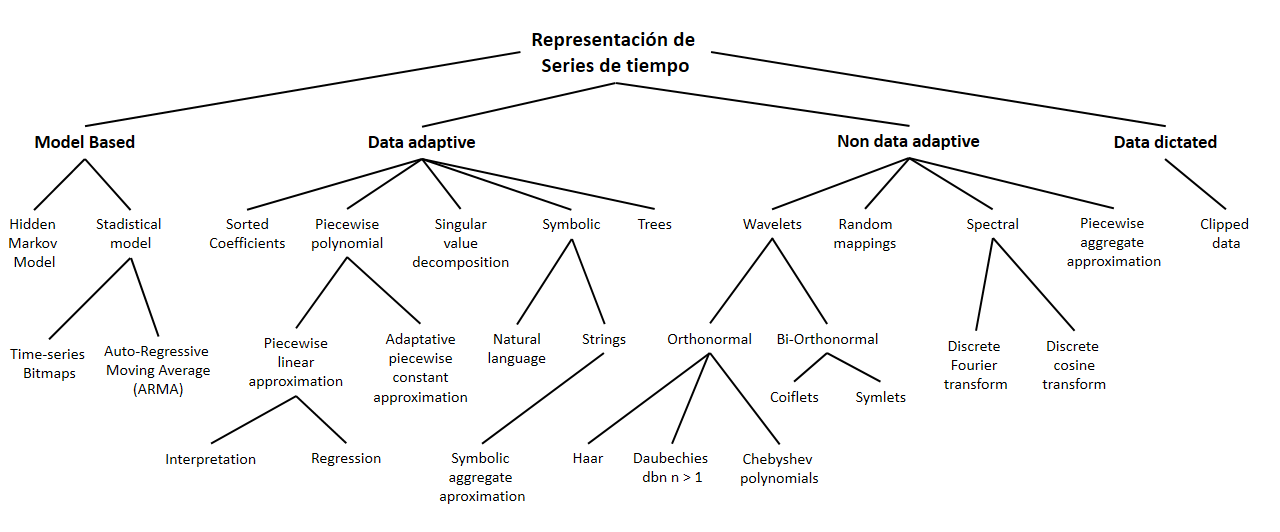
\includegraphics[width=1\textwidth]{imagenes/rst.png}
  \caption{Jerarqu�a de diferentes enfoques de representaci�n de series de tiempo}
  \label{fig:mesh1}
 \end{figure}

\subsubsection{Data adaptive}
Este enfoque implica que el par�metro de transformaci�n se ira modificando dependiendo de la naturaleza de los datos disponibles, en otras palabras usan una longitud no igual de segmentaci�n para la representaci�n de series de tiempo.

\textit{Symbolic Aggregate Approximation (SAX)}

Este m�todo de representaci�n permite una reducci�n de dimensionalidad de una longitud $n$ a otra cadena de caracteres de longitud $w$ donde se entiendo que siempre $w$ ser� menor que $n$, esta proceso de discretizaci�n usa como paso intermedio el algoritmo de representaci�n  Piecewise Aggregate Approximation
(PAA) para luego simbolizar esta representaci�n en un cadena discreta. Dado que una serie de tiempo tiene una distribuci�n Gaussiana \citep{rjam:2000:introduction} que es la base del algoritmo $SAX$, se puede determinar "breakpoints" que producir�n �reas $a$ de igual tama�o bajo la curva de Gaussinaa\citep{rjam:2000:introduction}, el algoritmo hace uso de los siguientes conceptos:

\begin{itemize}
  \item $Breakpoints$: los $Breakpoints$ �reas de igual tama�o que dividen una distribuci�n Gaussiana para ser aplicadas en $SAX$ estas valores ya est�n determinados en el siguiente (cuadro \ref{fig:bp}).
  \item $Word$: representan los s�mbolos que estar�n en cada intervalo del $Breakpoint$.
\end{itemize}

\begin{figure}[h]
  \centering
  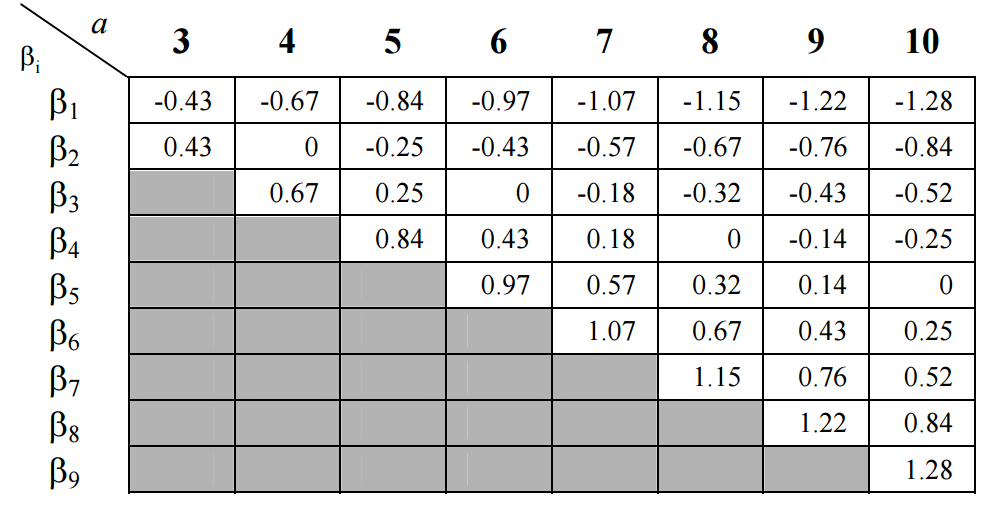
\includegraphics[scale=0.5]{imagenes/breakpoint.PNG}
  \caption{Una tabla de consulta que contiene los puntos de interrupci�n que dividen una distribuci�n de Gauss en un n�mero arbitrario (3-10) de las regiones equiprobables \protect\citep{lin:2007:experiencing}}
  \label{fig:bp}
\end{figure}

En la (figura \ref{fig:sax}) se muestRa un ejemplo gr�fico de como funciona $SAX$.

\begin{figure}[h]
  \centering
  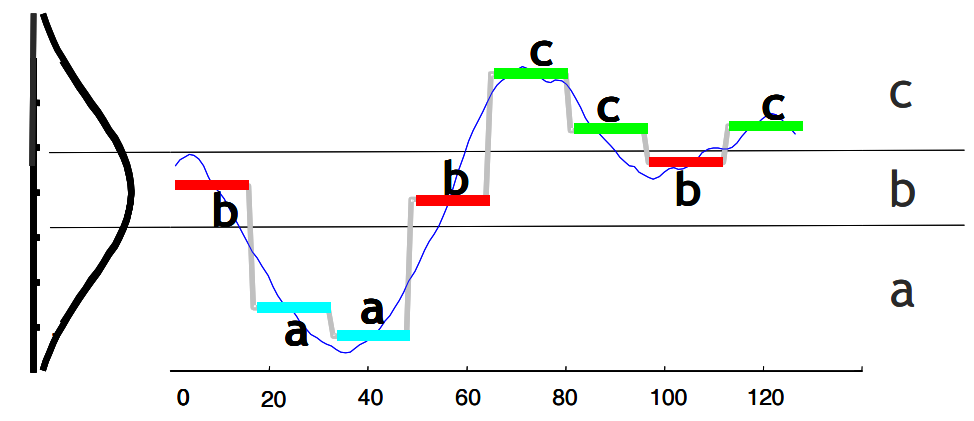
\includegraphics[scale=0.5]{imagenes/sax.PNG}
  \caption{Una serie de tiempo es discretizado mediante la obtenci�n de una primera aproximaci�n PAA y luego usando los $breakpoints$ predeterminados para asignar los coeficientes de PAA en s�mbolos SAX. \protect\citep{lin:2007:experiencing}}
  \label{fig:sax}
\end{figure}


\subsubsection{Non-data adaptive} 
los par�metros de la transformaci�n permanecen siendo los mismos para toda la serie de tiempo ignorando la naturaleza de la misma, en  \textit{Non-data adaptive} la longitud de la segmentaci�n es de igual longitud, algunos de estos m�todos son:

\textit{Piecewise Aggregate Approximation (PAA)}
  
En este m�todo, las series de tiempo se divide en segmentos k de igual longitud y luego cada segmento se sustituye con un valor constante, que es el valor medio del segmento. A continuaci�n, estos valores medios se agrupan en un vector, que representa la marca del segmento \citep{mitsa:2010:temporal}. Un ejemplo se muestra en la (Figura \ref{fig:paa}).


\begin{figure}[h]
  \centering
  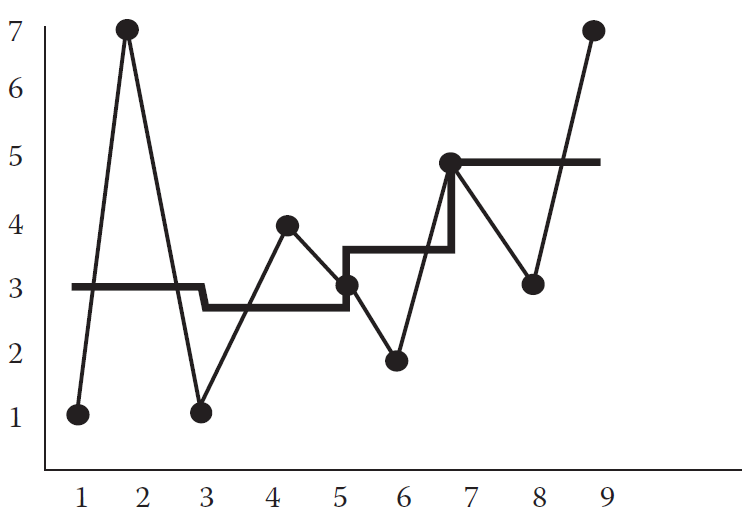
\includegraphics[scale=0.5]{imagenes/paa.PNG}
  \caption{Representaci�n PAA de una serie de tiempo}
  \label{fig:paa}
\end{figure}

Una definici�n m�s formal de PAA se da a continuaci�n, se tiene una serie de tiempo $C$ de longitud $n$ puede ser representado en un espacio de dimensi�n $w$ por un vector $\bar{C}=\bar{c_1},...,\bar{c_w}$. el elemento $i^{th}$ de $\bar{C}$ es calculado por la siguiente ecuaci�n:
\begin{equation}
\bar{c_i} = \frac{w}{n} \sum_{j = \frac{n}{w}(i-1)+1} ^{\frac{n}{w}i}c_j
\end{equation}
En pocas palabras, para reducir la serie de tiempo de $n$ dimensiones a $w$ dimensiones, los datos se divide en $w$ "marcos" de igual tama�o. El valor medio de los datos incluidos en una trama se calcula y un vector de estos valores se convierte en la representaci�n reducida de datos \citep{lin:2007:experiencing}.

\textit{Discrete Fourier Transform (DFT)}

Wavelets son m�s efectivos cuando la mayor�a de variaci�n in la serie puede ser capturado en una regi�n especifica local de la serie. En casos donde la serie contiene periodicidad global, el DFT es m�s efectivo \citep{Aggarwal:2015}.
El DFT representa una serie de tiempo en el dominio frecuencia, el coeficiente $F_k$ de una serie de tiempo $X={x_0,x_2,...,x_{n-1}}$ es un n�mero complejo dado por:

\begin{equation}
F_k = \sum_{i=0}^{N-1} x_i e^{-j2\pi ik/N}
\end{equation}
Donde: $k$ = 0, 1,...,N-1.

Una de las ventajas de usar DFT en procesamiento de se�ales es que existe un algoritmo r�pido para su calculo, conocido como
\textit{fast fourier transform} (FFT) su complejidad computacional es $O(n logn).$ 

\subsubsection{Model-based} 
Representan una series de tiempo de una forma estoc�stica, en estad�stica es un concepto matem�tico que sirve para tratar con magnitudes aleatorias o m�s exactamente para caracterizar una sucesi�n de variables aleatorias(estoc�sticas) que evolucionan en funci�n de otra variable, generalmente el tiempo.

\textit{Markov Models Representation}

modelos de Markov representan una serie de tiempo de una manera estoc�stica. \textit{Hidden Markov models} (HMM) son modelos de Markov cuyos par�metros son desconocidos. Una descripci�n detallada de los HMM se puede encontrar en \citep{rabiner:1989:tutorial}. Un HMM de primer orden se describe completamente con los siguientes par�metros:

\begin{itemize}
  \item El n�mero de estados.
  
  \item La distribuci�n de probabilidad de transici�n de estado, es decir, la probabilidad de que el sistema va a ir de un estado a otro.
  
  \item La densidad de las observaciones.
  
  \item La distribuci�n de probabilidad del estado inicial.
\end{itemize}

Para que un \textit{Hidden Markov models}  sea totalmente modelada probabil�sticamente, tenemos que especificar los estados anteriores y actuales. 

Un caso especial es una cadena de Markov, donde necesitamos saber s�lo el estado actual y predecesor. El problema de la estimaci�n de los par�metros de un HMM, dadas las observaciones, se puede ver como un problema de estimaci�n de m�xima verosimilitud. El problema, sin embargo, no tiene una soluci�n global.

algoritmos iterativos, tales como el algoritmo de Baum-Welch, s�lo se garantizan la convergencia a un m�ximo local. Los par�metros que se estiman por este algoritmo son la probabilidad del estado inicial, los par�metros de transici�n de estado, la media y la covarianza de la gaussiana de cada estado.


\subsubsection{Data dictated}
En este enfoque la tasa de comprensi�n es definido autom�ticamente de una serie de tiempo sin procesar \citep{tsclus_:decade_:review} tal como Clipped propuesto en \citep{ratanamahatana:2005:novel}.

\textit{The clipped representation}

En \citep{ratanamahatana:2005:novel} presenta el m�todo de representaci�n que trabaja remplazando cada dato del valor real por un �nico bit. como se muestra en la siguiente (figura \ref{fig:clipped}) 

\begin{figure}[h]
  \centering
  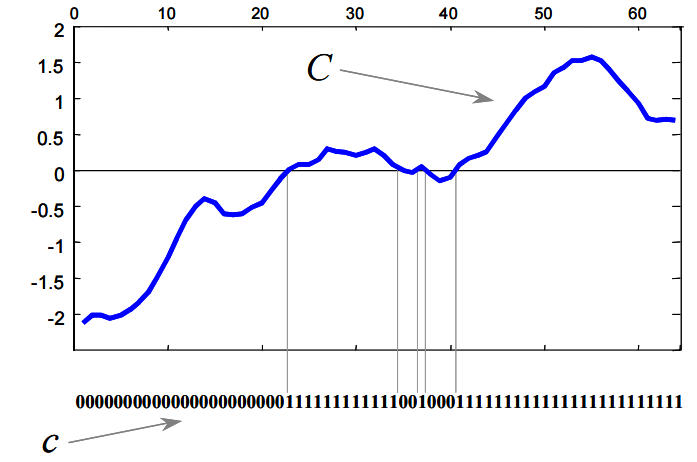
\includegraphics[scale=0.5]{imagenes/clipped.PNG}
  \caption{Una serie de tiempo de longitud 64, denotado por $C$, se convierte en la representaci�n $clipped$, denotado por $c$, simplemente observando los elementos de $C$, que los puntos encima de cero son 1 caso contrario son 0.}
  \label{fig:clipped}
\end{figure}

M�s formalmente, podemos definir $c$, la representaci�n $clipped$ de $C$ como:
\begin{equation}
c(i) = \begin{cases}1 & if \; \; \; C(i) > \mu\\0 & otherwise\end{cases}
\end{equation}

Donde $\mu$ es el valor medio de $C$, y en el caso que la serie de tiempo este normalizada se puede asumir que $\mu$ = 0.

%As you can see in the figure \ref{fig:mesh1}, the 
%function grows near 0. Also, in the page \pageref{fig:mesh1} 

%%%%%%%%%%%%%%%%%%%%%%%%%%%%%%%%%%%%%%%%%%%%%%%
\begin{comment}

\begin{table}[]
  \centering
  \caption{M�todos de representaci�n}
  \label{tab:metodosrep}
  \resizebox{\textwidth}{!}{%
    \begin{tabular}{@{}|l|l|l|l|l|@{}}
      \toprule
      \textbf{\begin{tabular}[c]{@{}l@{}}M�todos de\\ representaci�n\end{tabular}}                   & \textbf{Complejidad} & \textbf{Tipo}                                                                    & \textbf{Comentario}                                                                                                                                                                                                             & \textbf{\begin{tabular}[c]{@{}l@{}}Presentado\\ Por\end{tabular}} \\ \midrule
      \begin{tabular}[c]{@{}l@{}}Discrete Fourier \\ Transform (DFT)\end{tabular}                    & $O(n log(n))$        & \begin{tabular}[c]{@{}l@{}}Non data adaptive, \\ Spectral\end{tabular}           & \textbf{\begin{tabular}[c]{@{}l@{}}Uso: \\ Se�ales naturales\\ Pros:\\ Sin falsos despidos\\ Contra:\\ No soporta "time warped queries"\end{tabular}}                                                                           &                                                                   \\ \midrule
      \begin{tabular}[c]{@{}l@{}}Discrete Wavelet \\ Transform (DWT)\end{tabular}                    & $O(n)$               & \begin{tabular}[c]{@{}l@{}}Non data adaptive, \\ Wavelet\end{tabular}            & \textbf{\begin{tabular}[c]{@{}l@{}}Uso:\\ Se�ales estacionarias\\ Pros:\\ Mejores resultados que DFT\\ Contra:\\ Resultados no estables, \\ las se�ales deben tener una\\  longitud $ n=2^{alg\acute{u}nEntero} $\end{tabular}} &                                                                   \\ \midrule
      \begin{tabular}[c]{@{}l@{}}Singular Value \\ Decomposition (SVD)\end{tabular}                  & $O(Mn^{2})$          & Data adaptive                                                                    & \textbf{\begin{tabular}[c]{@{}l@{}}Pros:\\ Comunidad de procesamiento de texto\\ Contra:\\ Estructura de datos subyacente\end{tabular}}                                                                                         &                                                                   \\ \midrule
      \begin{tabular}[c]{@{}l@{}}Discrete Cosine \\ Transformation (DCT)\end{tabular}                &                      & \begin{tabular}[c]{@{}l@{}}Non data adaptive, \\ Spectral\end{tabular}           & \textbf{}                                                                                                                                                                                                                       &                                                                   \\ \midrule
      \begin{tabular}[c]{@{}l@{}}Piecewise Linear \\ Approximation (PLA)\end{tabular}                & $O(n\,log(n))$       & Data adaptive                                                                    & \textbf{\begin{tabular}[c]{@{}l@{}}Uso: \\ Se�ales naturales, biomedica\\ Contra:\\ No (actualmente) indexable, muy caro $O(n^2 N)$\end{tabular}}                                                                               &                                                                   \\ \midrule
      \begin{tabular}[c]{@{}l@{}}Piecewise Aggregate \\ Approximation (PAA)\end{tabular}             & $O(n)$               & Non data adaptive                                                                & \textbf{\begin{tabular}[c]{@{}l@{}}Uso:\\ Pros:\\ Contra:\end{tabular}}                                                                                                                                                         &                                                                   \\ \midrule
      \begin{tabular}[c]{@{}l@{}}Adaptive Piecewise \\ Constant Approximation \\ (APCA)\end{tabular} & $O(n)$               & Dada adaptive                                                                    & \textbf{\begin{tabular}[c]{@{}l@{}}Pros: \\ Muy eficiente\\ Contra:\\ compleja implementaci�n\end{tabular}}                                                                                                                     &                                                                   \\ \midrule
      \begin{tabular}[c]{@{}l@{}}Perceptually important \\ point (PIP)\end{tabular}                  &                      & Non data adaptive                                                                & \textbf{Uso: Finaciero}                                                                                                                                                                                                         &                                                                   \\ \midrule
      \begin{tabular}[c]{@{}l@{}}Chebyshev Polynomials \\ (CHEB)\end{tabular}                        &                      & \begin{tabular}[c]{@{}l@{}}Non data adaptive,\\ Wavalet Orthonormal\end{tabular} & \textbf{}                                                                                                                                                                                                                       &                                                                   \\ \midrule
      \begin{tabular}[c]{@{}l@{}}Symbolic Approximation\\ (SAX)\end{tabular}                         & $O(n)$               & Data adaptive                                                                    & \textbf{\begin{tabular}[c]{@{}l@{}}Uso:\\ Procesamiento de texto y bioinformatica\\ Pros:\\ Permite delimitaci�n inferior y reducci�n \\ de numerosidad  \\ Contra:\\ Discretizaci�n y tama�o del alfabeto\end{tabular}}        &                                                                   \\ \midrule
      Clipped Data                                                                                   &                      & Data dictated                                                                    & \textbf{\begin{tabular}[c]{@{}l@{}}Uso:\\ Hardware\\ Contra:\\ Representaci�n ultra compacto\end{tabular}}                                                                                                                      &                                                                   \\ \midrule
      \begin{tabular}[c]{@{}l@{}}Indexable Piecewise\\ Linear Approximation\\ (IPLA)\end{tabular}    &                      & Non data adaptive                                                                & \textbf{\begin{tabular}[c]{@{}l@{}}Uso:\\ Pros:\\ Contra:\end{tabular}}                                                                                                                                                         &                                                                   \\ \bottomrule
    \end{tabular}
    
  }
  
\end{table}
%%%%%%%%%%%%%%%%%%%%%%%%%%%%%%%%%%%%%%%%%%%%%%%%%
\end{comment}


\subsection {Medidas de similitud}
Las medidas de similitud son una tarea importante y adem�s la base de donde surgen t�cnicas m�s sofisticadas como la miner�a y an�lisis de series de tiempo, a diferencia del clustering tradicional donde una distancia entre objetos est�ticos es una comparaci�n exacta, en clustering en series de tiempo la distancia es calculada de manera aproximada. 
En el dominio de series de tiempo, la elaboraci�n de una funci�n de similitud apropiada no se hace de forma trivial. Hay esencialmente dos maneras en que los datos podr�an ser organizados y procesados \citep{agrawal:1993:efficient}, en \textit{whole series matching} donde se considera la longitud completa de toda la serie de tiempo durante la b�squeda de similitud. Se requiere la comparaci�n de la secuencia de consulta para cada serie candidata mediante la evaluaci�n de una funci�n de distancia y hacer el seguimiento de la secuencia con la distancia m�s peque�a \citep{fu:2011:review}. Esto problema de similitud puede ser resumido en dos formas \citep{mitsa:2010:temporal} de la siguiente manera:

\begin{enumerate}
  \item Encontrar todos los pares de series de tiempo que tienen una distancia que es menor que un n�mero $ n $.
  \item Indexaci�n y b�squeda de contenidos. Hay dos enfoques para este tipo de b�squeda: (1) por rango: Encuentre todas las series temporales que tienen distancia inferior a un n�mero $n$ a partir de una serie de tiempo espec�fica. (2) Busca los $m$ vecinos m�s cercanos para una serie de tiempo espec�fico.
\end{enumerate}
la otra manera es \textit{subsequence matching} donde una secuencia corta es comparada con una secuencia m�s larga, deslizando el anterior a lo largo de este ultimo. Una forma para calcular la distancia entre dos series de tiempo es consider�ndolos como series de tiempo univariadas, una serie de tiempo univariada es cuando solo tiene una dimensi�n que depende del tiempo, y luego calculando la medida de distancia a trav�s de todos los puntos.

La elecci�n de una medida de distancia depende netamente de las caracter�sticas de la serie de tiempo como son: la longitud, el m�todo de representaci�n y el objetivo del clustering \citep{tsclus_:decade_:review}, las medidas de distancia o similitud pueden ser divididas en cuatro categor�as \citep{esling:2012:time} que son las siguientes: 


\subsubsection{Shape-based:} 
compara en general la forma de las series de tiempo, los m�todos basados en esta categor�a son:

\textit{Dynamic Time Warping (DTW)}

Cuando se hace desea hacer una medida de similitud generalmente se asume que las dos series de tiempo que se quiere evaluar est�n alineadas en el eje-X, para solucionar este problema esta el algoritmos Dynamic Time Warping que consiste algoritmicamente como se explica en \citep{keogh:2001:derivative}: \\
Tenemos dos series de tiempo $Q$ Y $C$ de longitud $n$ y $m$ respectivamente donde: 

\begin{equation}
Q = q_1,q_2,...,q_i,...q_n
\end{equation}

\begin{equation}
Q = c_1,c_2,...,c_j,...c_m
\end{equation}

para alinear estas dos secuencias usando DTW se construye un matriz $n$ por $m$ donde el elemento $(i^{th},j^{th})$ de la matriz contiene las distancias $d(q_i,c_j)$ entre los dos puntos $q_i$ y $c_i$ (com�nmente se usa la distancia euclidiana as� que $d(q_i,c_j) = (q_i,c_j)^2$). cada elemento de la matriz $(i,j)$ corresponde a la alineaci�n entre los puntos $q_i$ y $c_j$. Esto se ilustra en la (figura \ref{fig:dtw}). Un  Warping path $W$ es un conjunto de elementos de la matriz que define un mapeo entre $Q$ Y $C$. El elemento $k^{th}$ de $W$ es definido como $w_k=(i,j)_k$ as� que tenemos:

\begin{equation}
W = w_1,w_2,...,w_k,...,w_k  \; \;   max(m,n) \leq  k < m+n+1
\end{equation}

El path warping esta sujeto a varias restricciones como son, condiciones de limites, continuidad, nonotonicidad, que est�n hechas para optimizar el rendimiento de su calculo.

\begin{figure}[h]
  \centering
  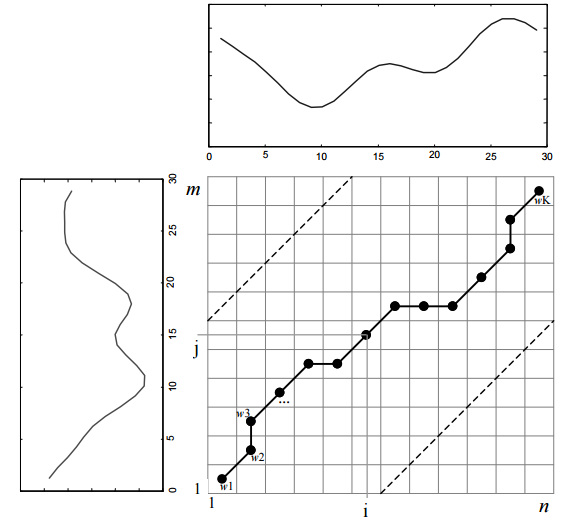
\includegraphics[scale=0.5]{imagenes/dtw.PNG}
  \caption{Ejemplo de \textit{warping path}}
  \label{fig:dtw}
\end{figure}

\textit{Spatial Assembling (SpADe)}

En este algoritmo, la similaridad es calculado por b�squeda de patrones coincidentes entre dos series de tiempo, El algoritmo \citep{chen:2007:spade} describe que teniendo dos secuencias $Q[0:m]$ y $D[0:n]$ de las cuales se extrae un conjunto de peque�os patrones de la serie de tiempo usando una ventaja deslizante de tama�o fijo. Esos peque�os patrones de una misma longitud son llamados patrones locales. Al utilizar el tama�o fijo de ventana deslizante en dos secuencias de tiempo, se obtienen dos conjuntos de patrones locales. \\

Un patr�n local $lp = (\theta_{pos}, \theta_{amp}, \theta_{shp}, \theta_{tscl}, \theta_{ascl})$, que son las que son la posici�n de $lp$ en $Q$ que significan:

\begin{itemize}
  \item $\theta_{pos}$: Es la posici�n de $lp$ en $Q$.
  \item $\theta_{amp}$: Es la amplitud media de los datos item en $lp$.
  \item $\theta_{shp}$: La forma que caracteriza de $lp$.
  \item $\theta_{tscl}$: La escala temporal de $lp$ (igual a 1 si $Q$ no esta escalado).
  \item $\theta_{ascl}$: La escala de amplitud de $lp$ (igual a 1 si $Q$ no esta escalado).
\end{itemize}

La distancia de los dos patrones locales $lp$ en $Q$ y $lp'$ en $D$, pueden ser medidos como:

\begin{equation}
D_1(lp', lp) = f(\mid \theta^{\:'}_{amp} - \theta^{\:'}_{amp} \mid, \mid \theta^{\:'}_{shp} - \theta^{\:'}_{shp} \mid)
\end{equation}

Que es una suma ponderada de las diferencias de las amplitudes y caracter�sticas de forma de los dos patrones locales, finalmente se procede a comparar estos patrones para hallar el grado de similitud.

\textit{DISSIM Distance}

Ha sido introducido para manejar la similitud de varias tasas de sampling. Esto es definido como una aproximaci�n de la integral de la distancia euclidiana que tambi�n se puede definir \citep{frentzos:2007:index} como:
La disimilaridad $DISSIM(Q,T)$ entre dos trayectorias $Q$ y $T$ que ha sido validado durante un periodo $[t_1, t_n]$ se expresa mediante la siguiente ecuaci�n:
\begin{equation}
DISSIM(Q,T) \approx \frac{1}{2}
\sum_{k=1}^{n-1}((D_{Q,T}(t_{k}) + D_{Q,T}(t_{k+1})) \cdot (t_{k+1} - t_k))
\end{equation}

Donde $D_{Q,T}(t)$ es una funci�n de la distancia euclidiana entre las trayectorias $Q$ Y $T$ con el tiempo.

\subsubsection{Edit-based:} 
compara dos series de tiempo en base al m�nimo n�mero de operaciones necesarias para transformar una serie a la otra.

\textit{Edit Distance with Real Penalty (ERP)} 

La distancia ERP es una medida de distancia el�stica para $matching$ en series de tiempo \citep{chen:2004:marriage}. Durante el calculo de la distancia ERP de dos series de tiempo $R$ y $S$ con longitudes $M$ y $N$, est�n alineados a la misma longitud mediante la adici�n de algunos s�mbolos (tambi�n llamados $gaps$) a ellos. A continuaci�n, cada elemento en una serie de tiempo o bien se corresponde con un $gap$ o un elemento en la otra serie de tiempo. finalmente la distancia ERP se define \citep{chen:2005:similarity}, dado dos series de tiempo $R$ y $S$ de longitud $M$ y $N$, respectivamente la distancia ERP de $R$ a $S$, $ERP(R,S)$, se define como:

\begin{equation}
ERP(R,S) = \begin{cases}
\sum_{i=1}^{M}|r_i-g| & if \;\;\; N= 0, \\
\sum_{i=1}^{N}|s_i-g| & if \;\;\; M = 0, \\
min
\begin{cases}
ERP(Rest(R),Rest(S)) + dist_{erp}(r_1, s_1),\\
ERP(Rest(R),S) + dist_{erp}(r_1, g),\\
ERP(R,Rest(S)) + dist_{erp}(s_1, g)
\end{cases} 
& otherwise
\end{cases}
\end{equation}

Donde:
\begin{equation}
dist_{erp}(r_i,s_i) = \begin{cases}
|r_i - s_i| & if \;\;\; r_i, s_i \; not \; gaps\\
|r_i - s_g| & if \;\;\; s_i \; is \;a\; gaps\\
|s_i - s_g| & if \;\;\; r_i \; is \;a\; gaps
\end{cases}
\end{equation}

y $g$ denota los $gap$ que se asigna un valor constante. 

\textit{The Longest Common Subsequence (LCSS)}

LCSS es una medida que es tolerante a la ausencia de puntos en la serie de tiempo(gaps) en las dos series que se quiere comparar, este algoritmo asume la misma base y escala para las dos series de tiempo y es superior a DTW en las siguientes aspectos \citep{vlachos:2003:indexing}:

\begin{itemize}
  \item LCSS maneja mejor el ruido y los $outliers$.
  \item El DTW puede distorsionar la distancia actual entre puntos en la serie de tiempo por $overfitting$.
  \item La complejidad computacional de DTW es significativa y adem�s su escalabilidad no es muy buena.
\end{itemize}

Una definici�n formal de LCSS la encontramos en \citep{loncomsub} y explica que teniendo dos secuencias de caracteres $X = {x_1,x_2,...,x_m}$ y $Z={z_1,z_2,...,z_k}$ decimos que $Z$ es una subsecuencia de $X$ si existe una secuencia estrictamente incremental de $k$ �ndices ${i_1,i_2,...,i_k}$ tal que $Z={X_{i1},X_{i2},...,X_{ik}}$, por ejemplo, tenemos $X={ABRACADABRA}$  y $Z={AADAA}$, luego $Z$ es una subsecuencia de $X$. \\

\subsubsection{Feature-based:} 
Se extraen las caracter�sticas describiendo aspectos de la serie que son luego comparadas con alg�n tipo de funci�n de distancia, entre los cuales tenemos los siguientes m�todos:

\textit{Autocorrelation Function}

Como se explica en \citep{correlationfun}, la funci�n de autocorrelaci�n(ACF) es una muy importante conjunto de caracter�sticas para el an�lisis de series de tiempo. Teniendo un conjunto de series de tiempo $X=[x_1,x_2,...,x_N]$ de longitud $N$ definimos un conjunto de caracter�sticas $Z$ de $M$-dimensiones como tambi�n un conjunto arbitrario de retardos (\textit{lags}) $k_1,k_2,...,k_M$. Tenemos $Z=[r_{k_1},r_{k_2},...,r_{k_M}]$, donde: 



\begin{equation}
r_k = \frac{1}{N} \sum_{i=1}^{N} x_ix_{[i+k]_N} 
\end{equation}

Donde los corchetes $[i-k]_N$ indican el modulo-$N$. Estos son conocidos como estimaciones ACF circular debido a la indexaci�n de m�dulo-$N$. Se elige esta forma de ACF porque simplifica el an�lisis. Finalmente se tiene el calculo de caracter�sticas como:

\begin{equation}
  Feature \; Calculation: \; Z = [r_{k_1},r_{k_2},...,r_{k_M}], \; Donde \; r_k = \frac{1}{N} \sum_{i=1}^{N} x_ix_{[i+k]_N} 
\end{equation}

Notar que es posible reescribir el calculo de las caracter�sticas como:

\begin{equation}
r_k = \frac{1}{N^2} \sum_{i=0}^{N/2} \epsilon_i y_i \cos\left\{ \frac{2\pi ik}{N}\right\}, \;\; k=0,1,...P,
\end{equation}
Donde $y={y_0,y_1,...,y_{N/2}}$ son los coeficientes DFT de magnitud al cuadrado, $\epsilon_i = 1$ para $i=0,N/2$, y $\epsilon_i = 2$ para $i=1, 2,...,N/2-1$.


\textit{Histogram distance}

Dado un conjunto de series de tiempo $D = {R_1,R_2,...,R_L}$, donde cada elemento $R$ esta representado por $R = [(r_1, t_1), . . . ,(r_N , t_N)]$ donde $N$ es el numero de puntos en $R_i$ y cada par de datos $(r, t)$ s�gnica tanto $r$ el valor en la marca de tiempo $t$. Para obtener el histograma del conjunto de datos $D$ se normaliza cada $R_i$ seg�n la formula mostrada en \citep{chen:2005:using}, luego los Histogramas son obtenidos dando un m�ximo $(max_D)$ y un m�nimo $(min_D)$, el rango $[nim_D, max_D]$ es dividido en $\tau$ subregiones de igual tama�o disjuntos, llamados $histogram bins$. Dado una serie de tiempo $R$, su histograma $H_R$ puede ser calculado por conteo de n�mero de puntos $h_i(1 \leq i \leq \tau$ que son ubicaciones en cada \textit{histogram \; bin} $ i: \; H_R = [h_1,...,h_{\tau}]$). Finalmente L1-norm o L2-norm \citep{swain:1991:color} pueden ser usados para medir la distancia entre dos histogramas.

\subsubsection{Structure-based:} 
Dividimos esta categor�a en dos subcategor�as espec�ficas. \textit{Model-based distances} que trabaja mediante el ajuste de un modelo para las diferentes series y, luego comparando los par�metros de los modelos subyacentes. \textit{Compression-based distances}. analizar qu� tan bien dos series se puede comprimir juntos. Similitud es reflejada por relaciones de compresi�n m�s altas.


\textit{Compression-based dissimilarity (CDM)}

Dado dos cadena de caracter�sticas, $x$ y $y$, definimos el $CDM$ como \citep{keogh:2007:compression}:
\begin{equation}
CDM(x,y) = \frac{C(xy)}{C(x) + C(y)}
\end{equation}
La disimilitud CDM se aproxima a 1 cuando $x$ e $y$ no est�n relacionados, y es m�s peque�o que 1 si $x$ e $y$ est�n relacionados. Cuanto menor sea el CDM $x$ e $y$ son m�s estrechamente relacionados aunque nunca ser� cero. El algoritmo comprime tanto la cadena $x$ como la cadena $y$, luego concatena las cadenas originales obteniendo $xy$ procediendo a comprimir, para aplicar finalmente la formula antes mencionada.

\begin{comment}
%****************************************
\begin{table}[]
  \centering
  \caption{Medidas de distancia}
  \label{tab:meddis}
  \begin{tabular}{llllllll}
    \hline
    \multicolumn{1}{|l|}{\textbf{Medida de distancia}}    & \multicolumn{1}{l|}{\textbf{E}} & \multicolumn{1}{l|}{\textbf{D}} & \multicolumn{1}{l|}{\textbf{R}} & \multicolumn{1}{l|}{\textbf{O}} & \multicolumn{1}{l|}{\textbf{M}} & \multicolumn{1}{l|}{\textbf{C}}   & \multicolumn{1}{l|}{\textbf{P}} \\ \hline
    \multicolumn{1}{|l|}{\textbf{Shape-based}}            & \multicolumn{1}{l|}{}           & \multicolumn{1}{l|}{}           & \multicolumn{1}{l|}{\textbf{}}  & \multicolumn{1}{l|}{}           & \multicolumn{1}{l|}{}           & \multicolumn{1}{l|}{}             & \multicolumn{1}{l|}{}           \\ \hline
    \multicolumn{1}{|l|}{Dynamic Time Warping (DTW)}      & \multicolumn{1}{l|}{}           & \multicolumn{1}{l|}{\checkmark} & \multicolumn{1}{l|}{\textbf{}}  & \multicolumn{1}{l|}{}           & \multicolumn{1}{l|}{}           & \multicolumn{1}{l|}{$O(n^2)$}     & \multicolumn{1}{l|}{1}          \\ \hline
    \multicolumn{1}{|l|}{Spatial Assembling (SpADe)}      & \multicolumn{1}{l|}{\checkmark} & \multicolumn{1}{l|}{\checkmark} & \multicolumn{1}{l|}{\checkmark} & \multicolumn{1}{l|}{}           & \multicolumn{1}{l|}{}           & \multicolumn{1}{l|}{$O(n^2)$}     & \multicolumn{1}{l|}{4}          \\ \hline
    \multicolumn{1}{|l|}{DISSIM}                          & \multicolumn{1}{l|}{}           & \multicolumn{1}{l|}{\checkmark} & \multicolumn{1}{l|}{\checkmark} & \multicolumn{1}{l|}{}           & \multicolumn{1}{l|}{\checkmark} & \multicolumn{1}{l|}{$O(n^2)$}     & \multicolumn{1}{l|}{0}          \\ \hline
    \multicolumn{1}{|l|}{\textbf{Edit-based}}             & \multicolumn{1}{l|}{}           & \multicolumn{1}{l|}{}           & \multicolumn{1}{l|}{\textbf{}}  & \multicolumn{1}{l|}{}           & \multicolumn{1}{l|}{}           & \multicolumn{1}{l|}{}             & \multicolumn{1}{l|}{}           \\ \hline
    \multicolumn{1}{|l|}{Edit with Real Penalty (ERP)}    & \multicolumn{1}{l|}{}           & \multicolumn{1}{l|}{\checkmark} & \multicolumn{1}{l|}{}           & \multicolumn{1}{l|}{\checkmark} & \multicolumn{1}{l|}{\checkmark} & \multicolumn{1}{l|}{$O(n^2)$}     & \multicolumn{1}{l|}{2}          \\ \hline
    \multicolumn{1}{|l|}{Longest Common SubSeq (LCSS)}    & \multicolumn{1}{l|}{}           & \multicolumn{1}{l|}{\checkmark} & \multicolumn{1}{l|}{\checkmark} & \multicolumn{1}{l|}{\checkmark} & \multicolumn{1}{l|}{}           & \multicolumn{1}{l|}{$O(n)$}       & \multicolumn{1}{l|}{2}          \\ \hline
    \multicolumn{1}{|l|}{Sequence Weighted Align (Swale)} & \multicolumn{1}{l|}{}           & \multicolumn{1}{l|}{\checkmark} & \multicolumn{1}{l|}{\checkmark} & \multicolumn{1}{l|}{\checkmark} & \multicolumn{1}{l|}{}           & \multicolumn{1}{l|}{$O(n)$}       & \multicolumn{1}{l|}{3}          \\ \hline
    \multicolumn{1}{|l|}{Edit Distance on Real (EDR)}     & \multicolumn{1}{l|}{}           & \multicolumn{1}{l|}{\checkmark} & \multicolumn{1}{l|}{\checkmark} & \multicolumn{1}{l|}{\checkmark} & \multicolumn{1}{l|}{\checkmark} & \multicolumn{1}{l|}{$O(n^2)$}     & \multicolumn{1}{l|}{2}          \\ \hline
    \multicolumn{1}{|l|}{\textbf{Feature-based}}          & \multicolumn{1}{l|}{}           & \multicolumn{1}{l|}{}           & \multicolumn{1}{l|}{\textbf{}}  & \multicolumn{1}{l|}{}           & \multicolumn{1}{l|}{}           & \multicolumn{1}{l|}{}             & \multicolumn{1}{l|}{}           \\ \hline
    \multicolumn{1}{|l|}{Autocorrelation}                 & \multicolumn{1}{l|}{}           & \multicolumn{1}{l|}{}           & \multicolumn{1}{l|}{\checkmark} & \multicolumn{1}{l|}{\checkmark} & \multicolumn{1}{l|}{\checkmark} & \multicolumn{1}{l|}{$O(nlogn)$}   & \multicolumn{1}{l|}{0}          \\ \hline
    \multicolumn{1}{|l|}{Threshold Queries (TQuest)}      & \multicolumn{1}{l|}{}           & \multicolumn{1}{l|}{\checkmark} & \multicolumn{1}{l|}{\checkmark} & \multicolumn{1}{l|}{\checkmark} & \multicolumn{1}{l|}{}           & \multicolumn{1}{l|}{$O(n^2logn)$} & \multicolumn{1}{l|}{1}          \\ \hline
    \multicolumn{1}{|l|}{Histogram}                       & \multicolumn{1}{l|}{}           & \multicolumn{1}{l|}{}           & \multicolumn{1}{l|}{\checkmark} & \multicolumn{1}{l|}{\checkmark} & \multicolumn{1}{l|}{\checkmark} & \multicolumn{1}{l|}{$O(n)$}       & \multicolumn{1}{l|}{0}          \\ \hline
    \multicolumn{1}{|l|}{\textbf{Structure-based}}        & \multicolumn{1}{l|}{}           & \multicolumn{1}{l|}{}           & \multicolumn{1}{l|}{}           & \multicolumn{1}{l|}{}           & \multicolumn{1}{l|}{}           & \multicolumn{1}{l|}{}             & \multicolumn{1}{l|}{}           \\ \hline
    \multicolumn{1}{|l|}{\textit{Model-based}}            & \multicolumn{1}{l|}{}           & \multicolumn{1}{l|}{}           & \multicolumn{1}{l|}{}           & \multicolumn{1}{l|}{}           & \multicolumn{1}{l|}{}           & \multicolumn{1}{l|}{}             & \multicolumn{1}{l|}{}           \\ \hline
    \multicolumn{1}{|l|}{Hidden Markov Models (HMM)}      & \multicolumn{1}{l|}{\checkmark} & \multicolumn{1}{l|}{\checkmark} & \multicolumn{1}{l|}{\checkmark} & \multicolumn{1}{l|}{\checkmark} & \multicolumn{1}{l|}{}           & \multicolumn{1}{l|}{$O(n^2)$}     & \multicolumn{1}{l|}{1}          \\ \hline
    \multicolumn{1}{|l|}{Auto-Regressive (ARMA)}          & \multicolumn{1}{l|}{}           & \multicolumn{1}{l|}{}           & \multicolumn{1}{l|}{\checkmark} & \multicolumn{1}{l|}{\checkmark} & \multicolumn{1}{l|}{}           & \multicolumn{1}{l|}{$O(n^2)$}     & \multicolumn{1}{l|}{2}          \\ \hline
    \multicolumn{1}{|l|}{\textit{Compression-based}}      & \multicolumn{1}{l|}{}           & \multicolumn{1}{l|}{}           & \multicolumn{1}{l|}{}           & \multicolumn{1}{l|}{}           & \multicolumn{1}{l|}{}           & \multicolumn{1}{l|}{}             & \multicolumn{1}{l|}{}           \\ \hline
    \multicolumn{1}{|l|}{Compression Dissimilarity (CDM)} & \multicolumn{1}{l|}{}           & \multicolumn{1}{l|}{\checkmark} & \multicolumn{1}{l|}{\checkmark} & \multicolumn{1}{l|}{\checkmark} & \multicolumn{1}{l|}{}           & \multicolumn{1}{l|}{$O(n)$}       & \multicolumn{1}{l|}{0}          \\ \hline
    &                                 &                                 &                                 &                                 &                                 &                                   &                                 \\
    &                                 &                                 &                                 &                                 &                                 &                                   &                                 \\
    &                                 &                                 &                                 &                                 &                                 &                                   &                                
  \end{tabular}
\end{table}
%***************************************

	\end{comment}

\begin{comment}
 \subsection{Clustering en Series de tiempo}
 Un cluster es un conjunto similar de objetos, donde la similaridad esta definida por una medida de distancia. El clustering representa un reto por los siguientes motivos \citep{mitsa:2010:temporal}:
 
 \begin{enumerate}
  \item Los valores de los atributos o caracter�sticas que diferencian un cluster de otro nos desconocidas.
  \item A diferencia de la clasificaci�n, no hay datos etiquetados. solo se puede tener un conocimiento a priori de un experto, esto lleva a su nombre de aprendizaje no supervizado en el campo de \textit{machine learning}.
  \item Debido a que no existe una gu�a en cuanto a lo que constituye un cl�ster, el �xito de los algoritmos de agrupamiento se ve influenciada por la presencia de ruido en los datos, los datos que faltan, y los valores at�picos. 
 \end{enumerate}
 
 Al igual que el clustering de datos est�ticos, clustering en series de tiempo requiere de algoritmos o procedimiento para formar clusters dado un conjunto de objetos de datos sin etiqueta, de tal forma la elecci�n del algoritmo de cluster depende tanto del tipo de datos disponibles y de la finalidad y aplicaci�n en particular \citep{liao:2005:clustering}. Para hacer �nfasis en la importancia y la necesidad de agrupar los conjuntos de datos de series de tiempo, pueden darse los siguientes objetivos para el agrupamiento de los datos de series de tiempo de la siguiente manera \citep{aghabozorgi:2015:time}:
 
 \begin{enumerate}
  \item Bases de datos de series temporales contienen informaci�n valiosa que se puede obtener a trav�s del descubrimiento de patrones. El clustering es una soluci�n com�n que se realiza para descubrir estos patrones en conjuntos de datos de series de tiempo.
  
  \item Clustering de series de tiempo es el m�todo m�s utilizado como una t�cnica de exploraci�n, y tambi�n como una subrutina en algoritmos de miner�a de datos m�s complejos, tales como el descubrimiento de reglas, indexaci�n, clasificaci�n y detecci�n de anomal�as \citep{chics:2009:clustering}.
  
  \item Representar las estructuras de clusters de series temporales como im�genes visuales (visualizaci�n de los datos de series de tiempo) puede ayudar a los usuarios a entender r�pidamente la estructura de datos, clusters, anomal�as y otras regularidades en los conjuntos de datos.
 \end{enumerate}
 
 El clustering en series de tiempo se define formalmente como:
 
 \begin{defi}
  (Clustering en Series de tiempo) dado un conjunto de datos de $n$ series de tiempo, datos $D = {F_1,F_2,...,F_n}$, el proceso de particionamiento sin supervisar de $D$ dentro de $C={C_1,C_2,...,C_k}$, de tal forma que series de tiempo homog�neas son agrupadas juntas basados en una medida de similitud, es llamado clustering de series de tiempo, luego $C_i$ es llamado un cluster, DONDE $D = \cup_{i=0}^k C_i$ y $C_i \cup C_j=\o$ para $i \neq j$.
 \end{defi}
 
 \subsubsection{Taxonom�a de clustering de series de tiempo}
 
 Existen dos categor�as en las cuales se clasifican la clusterizaci�n de series temporales \citep{esling:2012:time}, $whole series clustering$ y $subsequence clustering$
 
 \begin{itemize}
  \item \textit{Whole Series Clustering} 
  El clustering puede ser aplicar a cada serie de tiempo de un conjunto completo. El objetivo es reagrupar toda serie de tiempo en grupos de manera que las series de tiempo sean similares entre s� como sea posible dentro de cada grupo.
  \begin{defi}
    Dado una base de datos de series de tiempo $DB$ y una medida de similitud $D(Q,T)$, buscamos un conjunto de clusters $C={c_i}$ donde $c_i = {T_k | T_k \in DB}$ que maximiza la distancia entre clusters y miniminiza la variaci�n intracluster.
  \end{defi}
  
  \item \textit{Subsequence Clustering}
  Los clusters son creados por extracci�n de subsecuencias de una �nica o m�ltiples grandes series de tiempo.
  \begin{defi}
    Dado una serie de tiempo $T=(t_1,...,t_n)$ y una medida de similitud $D(Q,C)$, buscamos un conjunto de clusters $C={c_i}$ donde 
    $c_i = {T_j | T_j \in S_t^n}$ es un conjunto de subsecuencias que maximiza la distancia entre clusters y miniminiza la variaci�n intracluster.
  \end{defi}
  
 \end{itemize}
 
 Una revisi�n completa de toda la agrupaci�n de series de tiempo se lleva a cabo y se muestra en la Tabla 4. La revisi�n de la literatura, se observa que varias t�cnicas han sido recomendados para la agrupaci�n de los datos de series temporales enteros. Sin embargo, la mayor�a de ellos toman uno de los siguientes enfoques para agrupar los datos de series de tiempo:
 
 Como se vio antes hay dos formas de Clusterizar las series de tiempo, en $Whole series clustering$, en este forma de agrupamiento se muestran algunos enfoques \citep{tsclus_:decade_:review} que se toman para su procesamiento como se muestra en la (Imagen \ref{fig:enf}) 
 
 \begin{figure}[h]
  \centering
  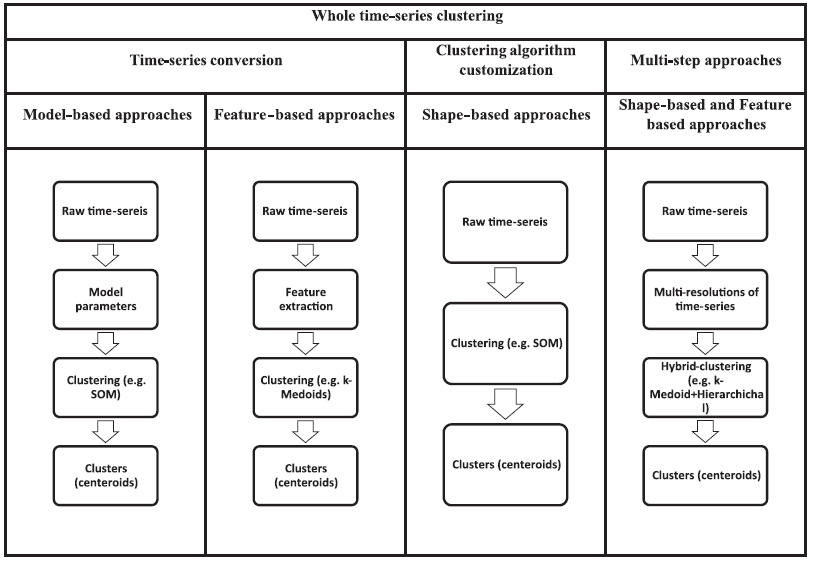
\includegraphics[scale=0.5]{imagenes/enfoques.PNG}
  \caption{Enfoques de clustering de series de tiempo}
  \label{fig:enf}
 \end{figure}
 
 \subsubsection{Clasificaci�n de los algoritmos de series de tiempo}
 
 El clustering de series de tiempo puede ser clasificado dentro de seis grupos: Particionamiento, Jerarquico, basados en grid, basados en modelo, basados en densidad y multi-step \citep{tsclus_:decade_:review}, \citep{rani:2012:recent}, \citep{liao:2005:clustering}.
 
 \textit{Clustering basados en particionamiento}
 
 La idea principal en esta clase de algoritmos de agrupamiento es crear $k$ cluster de los datos, donde el n�mero K es introducido por el usuario. Estos algoritmos son adecuados principalmente para datos num�ricos. La agrupaci�n original, tambi�n conocida como la partici�n, se lleva a cabo al azar y luego los objetos se mueven dentro y fuera de las agrupaciones, utilizando como gu�a un criterio de  "cercan�a". Los algoritmos de particionamiento son muy populares debido a su facilidad de implementaci�n y bajo costo computacional. Sin embargo, tienen estas desventajas: (1) que son sensibles a la presencia de ruido y los valores at�picos, (2) se pueden descubrir s�lo los cl�steres con formas convexas, y (3) el n�mero de grupos debe ser especificado \citep{esling:2012:time}. En el (cuadro \ref{tab:clus_particion}) presentamos los m�todos de particionamiento principales que hay en la literatura.
 
 % Please add the following required packages to your document preamble:
 % \usepackage{graphicx}
 % Please add the following required packages to your document preamble:
 % \usepackage{graphicx}
 \begin{table}[]
  \centering
  \resizebox{\textwidth}{!}{%
    \begin{tabular}{|l|l|l|l|l|}
      \hline
      \textbf{Algoritmo de clustering}                                             & \textbf{\begin{tabular}[c]{@{}l@{}}M�todo de \\ representaci�n\end{tabular}}                  & \textbf{\begin{tabular}[c]{@{}l@{}}Medida de \\ distancia\end{tabular}}              & \textbf{\begin{tabular}[c]{@{}l@{}}Comentario \\ (P:positivo, N: negativo)\end{tabular}} & \textbf{Applicaci�n}                                                                  \\ \hline
      k-means                                                                      & \begin{tabular}[c]{@{}l@{}}DWT\\  (Discrete Wavelet Transform) \\   Haar wavelet\end{tabular} & Euclidean                                                                            & \begin{tabular}[c]{@{}l@{}}P: Incremental \\ N: Sensitive to noise\end{tabular}          & *                                                                                     \\ \hline
      k-means                                                                      & \begin{tabular}[c]{@{}l@{}}BLA \\ (clipped timeseries representation)\end{tabular}            & LB\_clipped                                                                          & N: Sensitive to noise                                                                    & *                                                                                     \\ \hline
      k-Means                                                                      & DSA                                                                                           & DTW                                                                                  & N/A                                                                                      & *                                                                                     \\ \hline
      k-Means                                                                      & Shapelets                                                                                     & \begin{tabular}[c]{@{}l@{}}length-normalized \\ Euclidean distance\end{tabular}      & \begin{tabular}[c]{@{}l@{}}P: Cluster time-series \\ of different lengths\end{tabular}   & *                                                                                     \\ \hline
      K-Means                                                                      & *                                                                                             & \begin{tabular}[c]{@{}l@{}}CVT\\ (Computational Verb Theory)\end{tabular}            & *                                                                                        & Stock market data                                                                     \\ \hline
      K-Means                                                                      & *                                                                                             & Euclidean                                                                            & *                                                                                        & Portfolio management                                                                  \\ \hline
      K-Means                                                                      & *                                                                                             & N/A                                                                                  & *                                                                                        & Stock data                                                                            \\ \hline
      k-means                                                                      & Wavelet transform                                                                             & Kullback- Liebler divergence                                                         & *                                                                                        & \begin{tabular}[c]{@{}l@{}}Detection of activated \\ voxels in FMRI data\end{tabular} \\ \hline
      \begin{tabular}[c]{@{}l@{}}FCM \\ (Fuzzy c-Means Clustering)\end{tabular}    & Raw time-series                                                                               & \begin{tabular}[c]{@{}l@{}}Euclidean and \\ two cross correlation-based\end{tabular} & P: Noise Robustness                                                                      & *                                                                                     \\ \hline
      \begin{tabular}[c]{@{}l@{}}FCM\\ (Fuzzy c-Means Clustering)\end{tabular}     & (Fuzzy                                                                                        & c-Means                                                                              & Clustering)                                                                              & *                                                                                     \\ \hline
      \begin{tabular}[c]{@{}l@{}}FCM\\ (Fuzzy c-Means Clustering)\end{tabular}     & Raw time-series                                                                               & Euclidean Distance (ED)                                                              & P: Dynamic nature of algorithm                                                           & *                                                                                     \\ \hline
      \begin{tabular}[c]{@{}l@{}}FCM \\ (Fuzzy c-Means Clustering)\end{tabular}    & N/A                                                                                           & \begin{tabular}[c]{@{}l@{}}Euclidean and \\ two cross-correlation based\end{tabular} & *                                                                                        & \begin{tabular}[c]{@{}l@{}}Functional MRI brain \\ activity mapping\end{tabular}      \\ \hline
      \begin{tabular}[c]{@{}l@{}}PAM \\ (Partitioning Around Medoids)\end{tabular} & \begin{tabular}[c]{@{}l@{}}HMMs \\ (Hidden Markov Models)\end{tabular}                        & KL-Distance                                                                          & \begin{tabular}[c]{@{}l@{}}P: Support categorical \\ and continues values\end{tabular}   & *                                                                                     \\ \hline
      \begin{tabular}[c]{@{}l@{}}PAM \\ (Partitioning Around Medoids)\end{tabular} & AR                                                                                            & Euclidean                                                                            & *                                                                                        & Public data                                                                           \\ \hline
    \end{tabular}%
  }
  \caption{M�todos de clustering por particionamiento}
  \label{tab:clus_particion}
 \end{table}
 
 
 \textit{Clustering basados en Jerarqu�a}
 
 Como su nombre lo indica, en esta clase de algoritmos los objetos se colocan en una jerarqu�a ya sea en una de abajo hacia arriba (bottom-up) o de arriba hacia abajo (top-down) para crear los grupos. 
 La ventaja de este tipo de agrupamiento es que no requiere ning�n conocimiento sobre el n�mero de grupos, y su desventaja es su complejidad computacional \citep{lin:2004:visually}. Muy a menudo una estructura en forma de �rbol, un dendrograma, se utiliza para representados los niveles jer�rquicos anidados. 
 La mayor�a de los algoritmos jer�rquicos aglomerativas siguen un enfoque de abajo hacia arriba y comienzan con la formaci�n de cada objeto de su propia categor�a, en el (cuadro \ref{tab:clus_jerar}) mostramos los principales m�todos. 
 
 A continuaci�n, fusionamos estas agrupaciones en grupos cada vez m�s grandes hasta que se cumpla un criterio especificado de antemano, tales como el n�mero de grupos que se formen. Hay tres variaciones diferentes del algoritmo, en funci�n de c�mo se combinan grupos:
 
 Single link:  En este enfoque, dos grupos se fusionaron si la distancia m�nima entre dos objetos, uno de cada grupo, es menor o igual a una distancia de umbral predefinido.
 
 Average link: Aqu�, dos grupos se fusionan si la distancia media entre objetos en los dos grupos es menor que un umbral especificado previamente.
 
 Complete link: En este enfoque, dos grupos se fusionan si la distancia m�xima entre los puntos en los dos grupos es menor que o igual a un umbral especificado previamente. 
 
 % Please add the following required packages to your document preamble:
 % \usepackage{graphicx}
 \begin{table}[]
  \centering
  \resizebox{\textwidth}{!}{%
    \begin{tabular}{|l|l|l|l|l|}
      \hline
      \textbf{Algoritmo de clustering}                                       & \textbf{\begin{tabular}[c]{@{}l@{}}M�todo de \\ representaci�n\end{tabular}} & \textbf{\begin{tabular}[c]{@{}l@{}}Medida de \\ distancia\end{tabular}}                              & \textbf{\begin{tabular}[c]{@{}l@{}}Comentario \\ (P:positivo, N: negativo)\end{tabular}} & \textbf{Application}                                                         \\ \hline
      \begin{tabular}[c]{@{}l@{}}Agglomerative\\   hierarchical\end{tabular} & Raw time-series                                                              & J divergence                                                                                         & \begin{tabular}[c]{@{}l@{}}P: Multiple variable \\ support\end{tabular}                  & \begin{tabular}[c]{@{}l@{}}Earthquakes and \\ mining explosions\end{tabular} \\ \hline
      \begin{tabular}[c]{@{}l@{}}Agglomerative\\   hierarchical\end{tabular} & Raw time-series                                                              & Root mean square                                                                                     & \begin{tabular}[c]{@{}l@{}}N: Single variable, \\ using raw time-series\end{tabular}     & \begin{tabular}[c]{@{}l@{}}Daily power \\ consumption\end{tabular}           \\ \hline
      \begin{tabular}[c]{@{}l@{}}Agglomerative\\   hierarchical\end{tabular} & Raw time-series                                                              & \begin{tabular}[c]{@{}l@{}}Gaussian models \\ of data errors\end{tabular}                            & -                                                                                        & \begin{tabular}[c]{@{}l@{}}Seasonality pattern \\ in retails\end{tabular}    \\ \hline
      \begin{tabular}[c]{@{}l@{}}Agglomerative\\   hierarchical\end{tabular} & Raw time-series                                                              & \begin{tabular}[c]{@{}l@{}}Kullback�??Leibler \\ discrimination information \\ Measures\end{tabular} & \begin{tabular}[c]{@{}l@{}}P: Multiple \\ variable support\end{tabular}                  & \begin{tabular}[c]{@{}l@{}}Earthquakes and \\ mining explosions\end{tabular} \\ \hline
      \begin{tabular}[c]{@{}l@{}}Agglomerative\\   hierarchical\end{tabular} & *                                                                            & Euclidean                                                                                            & *                                                                                        & \begin{tabular}[c]{@{}l@{}}Flow velocity in \\ a wind tunnel\end{tabular}    \\ \hline
      \begin{tabular}[c]{@{}l@{}}Agglomerative\\   hierarchical\end{tabular} & \begin{tabular}[c]{@{}l@{}}Hierarchical \\ smoothing models\end{tabular}     & \begin{tabular}[c]{@{}l@{}}Unknown \\ (most likely Euclidean)\end{tabular}                           & *                                                                                        & Music performance                                                            \\ \hline
      \begin{tabular}[c]{@{}l@{}}Agglomerative\\   hierarchical\end{tabular} & AR(�??)                                                                      & Euclidean                                                                                            & *                                                                                        & \begin{tabular}[c]{@{}l@{}}Industrial \\ production indices\end{tabular}     \\ \hline
      Hierarchical                                                           & SAX                                                                          & \begin{tabular}[c]{@{}l@{}}Compression-based \\ distance\end{tabular}                                & N: Sensitive to noise                                                                    & *                                                                            \\ \hline
      Hierarchical                                                           & PCA                                                                          & SpCA Factor                                                                                          & \begin{tabular}[c]{@{}l@{}}P: Anomaly detection \\ N: Sensitive to noise\end{tabular}    & *                                                                            \\ \hline
      Hierarchical                                                           & Raw time-series                                                              & triangle distance                                                                                    & ?                                                                                        & *                                                                            \\ \hline
      Single-linkage                                                         & Raw time-series                                                              & Ad hoc distance                                                                                      & \begin{tabular}[c]{@{}l@{}}N: using raw time-series \\ Sensitive to noise\end{tabular}   & *                                                                            \\ \hline
    \end{tabular}%
  }
  \caption{M�todos de clustering Jer�rquicos}
  \label{tab:clus_jerar}
 \end{table}
 
 \textit{Clustering basados en densidad}
 
 En esta clase de algoritmos, la idea principal es mantener creciendo los cluster, siempre y cuando su densidad es superior a un cierto umbral.  La ventaja de los algoritmos basados en la densidad, en comparaci�n con los algoritmos de partici�n que se basan distancia, es que pueden detectar grupos de forma arbitraria, en la (tabla \ref{tab:clus_densidad}) se muestran algunos m�todos de clustering basados en densidad.
 
 
 % Please add the following required packages to your document preamble:
 % \usepackage{graphicx}
 \begin{table}[]
  \centering
  \resizebox{\textwidth}{!}{%
    \begin{tabular}{|l|l|l|}
      \hline
      \textbf{Algorithm}                                                               & \textbf{Distance Measure} & \textbf{Application}                \\ \hline
      \begin{tabular}[c]{@{}l@{}}Density Based Subsequence\\   Clustering\end{tabular} & Dynamic Time Warping      & Detecting climate change            \\ \hline
      Kernal DBScan                                                                    & Euclidean                 & Multivariate time series clustering \\ \hline
    \end{tabular}%
  }
  \caption{M�todos de clustering basados en densidad}
  \label{tab:clus_densidad}
 \end{table}
 
 \textit{Clustering basados en Modelos}
 
 Clustering basados en modelos intenta recuperar el modelo original a partir de un conjunto de datos. Este enfoque supone un modelo para cada grupo, y encuentra el mejor ajuste de los datos a ese modelo. En detalle, se da por supuesto que hay algunas centroides elegidos al azar, y luego se a�ade un poco de ruido a ellos con una distribuci�n normal. El modelo que se recupera de los datos generados define grupos \citep{Shavlik:1991}. Por lo general, los m�todos basados en modelos utilizan m�todos estad�sticos como lo muestra el (cuadro \ref{tab:clus_model}).
 
 % Please add the following required packages to your document preamble:
 % \usepackage{graphicx}
 \begin{table}[]
  \centering
  \resizebox{\textwidth}{!}{%
    \begin{tabular}{|l|l|l|l|}
      \hline
      \textbf{Clustering Algorithm}                                                                                                                          & \textbf{\begin{tabular}[c]{@{}l@{}}Representation \\ method\end{tabular}} & \textbf{\begin{tabular}[c]{@{}l@{}}Distance \\ Measure\end{tabular}}                                                    & \textbf{Application}                                                             \\ \hline
      Modified SOM                                                                                                                                           & \begin{tabular}[c]{@{}l@{}}Perceptually\\ important points\end{tabular}   & \begin{tabular}[c]{@{}l@{}}Sum of the mean squared \\ distance along thebvertical and \\ horizontal scales\end{tabular} & \begin{tabular}[c]{@{}l@{}}Hong Kong \\ stock market\end{tabular}                \\ \hline
      EM learning                                                                                                                                            & Gaussian mixture                                                          & Log-likelihood                                                                                                          & Non-specific                                                                     \\ \hline
      EM learning                                                                                                                                            & Discrete HMM                                                              & Log-likelihood                                                                                                          & \begin{tabular}[c]{@{}l@{}}Tool \\ conditionmonitoring\end{tabular}              \\ \hline
      EM learning                                                                                                                                            & ARMA mixture                                                              & Log-likehood                                                                                                            & Public data                                                                      \\ \hline
      \begin{tabular}[c]{@{}l@{}}Forward propagation\\   learning algorithm\end{tabular}                                                                     & Empirical mode decomposition                                              & Euclidean                                                                                                               & Non-specific                                                                     \\ \hline
      \begin{tabular}[c]{@{}l@{}}Neural network clustering\\   performed by a batch EM \\ version of minimal free energy \\ vector quantization\end{tabular} & *                                                                         & N/A                                                                                                                     & \begin{tabular}[c]{@{}l@{}}Functional MRI \\ brain activity mapping\end{tabular} \\ \hline
    \end{tabular}%
  }
  \caption{M�todos de clustering basados en modelos}
  \label{tab:clus_model}
 \end{table}
 
 
 \textit{Clustering basados en Grid}
 
 Los m�todos basados en cuadricula $(grid)$ cuantifican el espacio en un n�mero finito de celdas que forman una cuadricula, y luego realizar la agrupaci�n en las celdas de la cuadr�cula, no se han encontrado muchos trabajos aplicados en series de tiempo, los existentes son mostrados en la (tabla \ref{tab:clus_grid}).
 
 % Please add the following required packages to your document preamble:
 % \usepackage{graphicx}
 \begin{table}[]
  \centering
  \resizebox{\textwidth}{!}{%
    \begin{tabular}{|l|l|l|l|l|}
      \hline
      \textbf{Paper} & \textbf{Features} & \textbf{Distance Measure} & \textbf{Clustering Algorithm}  & \textbf{Application}  \\ \hline
      Dong Jixue     & Wavelet transform & N/A                       & Grid-based partitioning method & Financial time-series \\ \hline
    \end{tabular}%
  }
  \caption{M�todos de clustering basados en grid}
  \label{tab:clus_grid}
 \end{table}
 
 \textit{Clustering basados en M�ltiples Pasos}
 
 Aunque hay muchos estudios para mejorar la calidad de los enfoques de representaci�n, la medici�n de distancia, etc, unos pocos art�culos hacen �nfasis en algoritmos que mejoran y presentar un nuevo modelo (por lo general como un m�todo h�brido) para la agrupaci�n de los datos de series temporales. los m�todos se resumen en la (tabla \ref{tab:clus_multi}).
 
 % Please add the following required packages to your document preamble:
 % \usepackage{graphicx}
 \begin{table}[]
  \centering
  \resizebox{\textwidth}{!}{%
    \begin{tabular}{|l|l|l|l|}
      \hline
      \textbf{Algoritmo de clustering}                                                    & \textbf{\begin{tabular}[c]{@{}l@{}}M�todo de \\ representaci�n\end{tabular}}       & \textbf{\begin{tabular}[c]{@{}l@{}}Medida de \\ distancia\end{tabular}}                & \textbf{\begin{tabular}[c]{@{}l@{}}Comentario \\ (P:positivo, N: negativo)\end{tabular}}                                                                      \\ \hline
      \begin{tabular}[c]{@{}l@{}}Partitioning clustering,\\   k-Means and EM\end{tabular} & Wavelets                                                                           & Euclidean Distance                                                                     & \begin{tabular}[c]{@{}l@{}}P: Incremental \\ N: Sensitive to noise\end{tabular}                                                                               \\ \hline
      two stages approach                                                                 & Raw time-series                                                                    & \begin{tabular}[c]{@{}l@{}}GLR \\ (generalized likelihood ratio)\end{tabular}          & \begin{tabular}[c]{@{}l@{}}N: Subsequence Segmentation. \\ Sensitive to noise\end{tabular}                                                                    \\ \hline
      \begin{tabular}[c]{@{}l@{}}Two-level clustering:\\   CAST,CAST\end{tabular}         & SAX, Raw time-series                                                               & \begin{tabular}[c]{@{}l@{}}Min-Dist, \\ Eucleadian distance\end{tabular}               & \begin{tabular}[c]{@{}l@{}}P: Support unequal time-series \\ N: Based on subsequence,\\ CAST is poor in front of huge \\ data Sensitive to noise\end{tabular} \\ \hline
      \begin{tabular}[c]{@{}l@{}}Hybrid,\\   k-Medoids+Hierarchical\end{tabular}          & \begin{tabular}[c]{@{}l@{}}PAA \\ (Piecewise Aggregate Approximation)\end{tabular} & \begin{tabular}[c]{@{}l@{}}Euclidean distance and \\ Dynamic Time Warping\end{tabular} & \begin{tabular}[c]{@{}l@{}}P: Better accuracy over traditional\\   clustering algorithms\end{tabular}                                                         \\ \hline
    \end{tabular}%
  }
  \caption{M�todos de clustering basados en multiples pasos}
  \label{tab:clus_multi}
 \end{table}
\end{comment}


\section{Evoluci�n temporal de temas}\label{sec:nui_mt}

\section{Proyecci�n de datos multi-dimensionales}\label{sec:nlp_mt}
Debido al incremento de datos, no solo en el n�mero de registros, sino tambi�n en las dimensiones que poseen, como por ejemplo un vector de caracter�sticas de un documento, el vector caracter�stica estar� conformado por el n�mero de ocurrencias de cada palabra que contiene de tal forma si tenemos $m$ atributos se tendr� un vector $m$ dimensional.

M�todos convencionales de visualizaci�n de datos fallan cuando son aplicados directamente sobre datos de alta dimensionalidad como en el caso de identificaci�n de patrones \citep{berkhin2006survey}.

Una forma de manejar esta alta dimensionalidad de forma que puedan ser visualizadas de forma correcta son las \textit{proyecciones multidimensionales}, estas t�cnicas permiten reducir la dimensionalidad de un espacio original $m$ a uno espacio $p$-dimensional donde $p$ $\ll$ $m$ pudiendo ser las dimensiones de $p$: ${1,2,3}$, ademas logran conservar en lo mas posible las relaciones de distancia del espacio original 

\begin{defi}
	(Proyecci�n Multidimensional \citep{tejadaimproved}) Sea $X$ un conjunto de objetos en  $\mathbb{R}^{m}$ con $\updelta$ : $\mathbb{R}^m$ $x$ $\mathbb{R}^m$ $\longrightarrow$ $\mathbb{R}$ un criterio de proximidad entre objetos en $\mathbb{R}^m$, y $Y$ un conjunto de puntos en $\mathbb{R}^p$ para $p={1,2,3}$ y $d$ : $\mathbb{R}^p$ $x$ $\mathbb{R}^p$ $\longrightarrow$ $\mathbb{R}$ un criterio de proximidad en $\mathbb{R}^p$. Una t�cnica de proyecci�n multidimensional puede ser descrita como una funci�n $f:X \longrightarrow X$ cuyo objetivo es hacer $\mid \updelta(x_i,x_j)-d(f(x_i),f(x_j)) \mid$ o mas proximo posible a cero, $\forall x_i, x_j \in X$.
\end{defi}

\subsection{T�cnicas de proyecciones de datos multidimensionales}
Existen variedad de t�cnicas aplicadas a diferentes campos para la realizar proyecciones multidimensionales, seg�n \citep{tejadaimproved} se pueden clasificar en tres grandes grupos: (1) \textit{Force-Direct Placement(FDP)}; (2) \textit{Multidimensional Scaling(MDS)}; y (1) \textit{T�cnicas para reducci�n de dimensionalidad}.

\section{�rboles filo-gen�ticos}\label{sec:dbs_mt}


%\citep{131:yoh:2001}
%Figura \ref{fig:2d-3d-vr}
%\begin{figure}[h]
% \centering
% \subfigure[]
% {
%   \includegraphics[width=0.45\columnwidth]{imagenes/bugarium.png}
%   \label{fig:2d}
% }
% \subfigure[]
% {
%   \includegraphics[width=0.45\columnwidth]{imagenes/unifiedcity.png}
%   \label{fig:3d}
% }
% \subfigure[]
% {
%   \includegraphics[width=0.45\columnwidth]{imagenes/teleinmersive.png}
%   \label{fig:vr}
% }
% \caption{Tipos de representaciones de informaci�n. (a) Representaci�n 2D - Bugarium \citep{018:yongpisanpop:2014}. (b) Representaci�n 3D - UnifiedCity \citep{152:teyseyre:2009}. (c) Representaci�n RV - Tele Inmersive Data Explorer.\citep{115:sawant:2000}}
% \label{fig:2d-3d-vr}
%\end{figure}
%\chapter{Desarrollo}

\section{Configuraci�n F�sica del Entorno Inmersivo}%\label{sec:vr_mt}

\subsection{Uni�n de Dispositivos al Ordenador}

Como primer avance se realiz� la configuraci�n de los equipos (Figura \ref{fig:configuracion}). El \textit{Leap Motion} fue adherido en la parte frontal del \textit{Oculus Rift}, luego ambos equipos fueron conectados a una \textit{Laptop} v�a dos puertos \textit{USB} y un puerto \textit{HDMI}. En cuanto a la configuraci�n \textit{software}, se instal� el motor de gr�ficos \textit{Unity3D} en su versi�n 5.02, el cual es gratuito para fines no comerciales. 

\begin{figure}[h!]
	\centering
	\subfigure[]
	{
		\includegraphics[width=0.41\columnwidth]{imagenes/esquema-1.png}
		\label{fig:esquema1}
	}
	\subfigure[]
	{
		\includegraphics[width=0.44\columnwidth]{imagenes/esquema-2.png}
		\label{fig:esquema2}
	}
	\caption{Configuraci�n del entorno inmersivo. (a) Esquema de configuraci�n. (b) Funcionamiento real del entorno virtual inmersivo}
	\label{fig:configuracion}
\end{figure}

\section{Construcci�n del Ambiente Virtual}

Para determinar las principales directrices para la construcci�n de un entorno virtual inmersivo, adecuado para la exploraci�n de art�culos cient�ficos, se ha realizado una extensa revisi�n de la literatura, recopilando las directrices y recomendaciones para la elaboraci�n de un buen entorno inmersivo.

\subsection{Directrices para la Construcci�n del Entorno Virtual}

Las principales directrices son:

\begin{itemize}
	\item \textbf{Simplicidad} para evitar sobrecargar la interfaz, s�lo se deben de utilizar los elementos necesarios. De esta forma se facilita las tareas de percepci�n y cognici�n al usuario.
	
	\item \textbf{Fondo oscuro}, para mitigar el mareo disminuyendo la frecuencia de actualizaci�n requerida para la rotaci�n del observador.

	\item \textbf{L�neas blancas}, delimitadoras del ambiente virtual, los cuales permiten al usuario percibir la profundidad con mayor precisi�n.

    \item \textbf{Rango de colores cercano a lo real}, para evitar el Efecto de TDF, que indica que si las im�genes no se perciben como reales, causan mareo y una serie de malestares.
    
    \item \textbf{Elementos redondeados}, se ajustan mejor a la forma de la mano y permiten que se generen sobras degradadas que facilitan su visualizaci�n.

	\item \textbf{Visualizaci�n del avatar de AliciaVR}, para fines de aumentar el sentido de presencia del usuario en el ambiente.

\end{itemize}
\begin{figure}[h]
	\centering
	\includegraphics[width=0.80\columnwidth]{imagenes/entorno2.png}
	\caption{Construcci�n del Entorno.}
	\label{%*fig:tmp
	}
\end{figure}

\subsection{Elaboraci�n del Avatar de Alicia}

Para que el usuario se imagine quien es su asistente, es que se implementa un avatar para la base de datos cient�fica ALICIA. Este avatar debe poseer caracter�sticas humanas, pero sin llegar a parecer un humano completamente. De esta forma se busca lograr que el usuario intuya que puede interactuar mediante comandos de voz. 

Es importante se�alar que el avatar no es un robot con inteligencia artificial, pero si posee las funciones b�sicas dentro del contexto de la exploraci�n de art�culos cient�ficos.

\begin{figure}[h]
	\centering
	\includegraphics[width=0.6\columnwidth]{imagenes/tmp9.png}
	\caption{Avatar de ALICIA de la interfaz AliciaVR.}
	\label{%*fig:tmp
	}
\end{figure}


\section{An�lisis e Implementaci�n de la Interacci�n Natural}

\subsection{Implementaci�n de la interacci�n b�sica}

Posterior a la configuraci�n del entorno inmersivo, se procedi� a investigar las t�cnicas de interacci�n para entornos virtuales inmersivos, empezando por el primer grupo de ``Exploraci�n Visual'', el cual comprende a la t�cnica de selecci�n. 

\begin{itemize}
	\item Experimento 1. T�cnica de Selecci�n: Manipulaci�n Directa.
	
	En esta t�cnica, la selecci�n de objetos se realiza mediante el empleo de una mano virtual, que copia exactamente los movimientos de la mano real. Para seleccionar un elemento se lo debe sostener del mismo modo como se har�a en el mundo real. En esta t�cnica de selecci�n, los elementos deben poseer propiedades s�lidas y f�sicas para una mejor interacci�n. En la Figura \ref{fig:seleccion0} se muestra la selecci�n de un nodo por manipulaci�n directa, como se puede apreciar, es id�ntico a agarrar un objeto del mundo f�sico. 
	
	\begin{figure}[h!]
		\centering
		
		\includegraphics[width=0.45\columnwidth]{imagenes/seleccion0.png}
		
		
		\caption{Ejemplo de selecci�n por manipulaci�n directa de un nodo.}
		\label{fig:seleccion0}
	\end{figure}
	
	\item Experimento 2. T�cnica de Selecci�n: Manipulaci�n por Gestos.
	
	La manipulaci�n por gestos consiste en seleccionar elementos en el entorno inmersivo mediante gestos con la mano virtual. Espec�ficamente para agarrar un objeto se debe realizar el gesto de `Pinch', basada en la met�fora del pellizco, y para soltar el elemento se debe de realizar el gesto de `Stop', que consiste en colocar la palma abierta. 
	
	En la Figura \ref{fig:select1} el nodo es seleccionado con el primer gesto descrito, luego en la Figura \ref{fig:select2} el nodo deja de estar seleccionado mediante el segundo gesto. Esta t�cnica no es del todo intuitiva, debido a que ambos gestos para el usuario pueden tener otro significado o al realizarlos pueden esperar realizar una acci�n diferente.
	
	\begin{figure}[h!]
		\centering
		\subfigure[]
		{
			\includegraphics[width=0.40\columnwidth]{imagenes/seleccion1.png}
			\label{fig:select1}
		}
		\subfigure[]
		{
			\includegraphics[width=0.40\columnwidth]{imagenes/seleccion2.png}
			\label{fig:select2}
		}
		\caption{Ejemplo de selecci�n por gestos de un nodo. (a) Selecci�n del elemento. (b) Des-selecci�n del elemento.}
		\label{fig:seleccion-12}
	\end{figure}
	
	\item Experimento 3. T�cnica de Selecci�n: Manipulaci�n Artificial.
	
	Esta t�cnica fue propuesta aprovechando la propiedad del mundo virtual que permite, previa configuraci�n, atravesar los objetos. Por tanto, para seleccionar un objeto solo es necesario atravesarlo utilizando la mano virtual. Para dejar de seleccionar el elemento solo se requiere atravesarlo nuevamente. 
	
	En la Figura \ref{fig:select3} el cubo es seleccionado cambiando de color a verde y en la Figura \ref{fig:select4} el cubo regresa a su estado anterior.
	
	\begin{figure}[h!]
		\centering
		\subfigure[]
		{
			\includegraphics[width=0.40\columnwidth]{imagenes/seleccion3.png}
			\label{fig:select3}
		}
		\subfigure[]
		{
			\includegraphics[width=0.40\columnwidth]{imagenes/seleccion4.png}
			\label{fig:select4}
		}
		\caption{Ejemplo de selecci�n por manipulaci�n artificial de un nodo. (a) Selecci�n del nodo. (b) Des-selecci�n del nodo.}
		\label{fig:seleccion-34}
	\end{figure}
	
\end{itemize}

\section{Implementaci�n del Web Crawler para la Recuperaci�n de Informaci�n de Alicia}

El modelo de interfaz propuesto (AliciaVR) est� conectado con la base de datos cient�fica ALICIA, para recuperar informaci�n de este sistema inform�tico se desarrollar� e implementar� un programa del tipo rastreador que se comunicar� autom�ticamente con ALICIA y extraer�, mediante an�lisis del c�digo fuente de sus vista, la informaci�n que necesitamos para visualizar en nuestra interfaz basada en realidad virtual.

Para lo cual se utiliz� la librer�a \textit{Barebones Ultima Web Crawler} y el servidor web \textit{Wamp Server 5.02} instalado en modo local.

La implementaci�n implica estudiar el patr�n adecuado para realizar el rastreo y extracci�n de recuperaci�n de forma automatizada, en la Figura \ref{fig:codigocrawler} se muestra un fragmento del c�digo fuente del rastreador escrito en el lenguaje \textit{PHP}.

\begin{figure}[h]
	\centering
	\includegraphics[width=0.7\columnwidth]{imagenes/crawlercod.png}
	\caption{Web Crawler Configuraci�n.}
	\label{fig:codigocrawler}
\end{figure}

La activaci�n del rastreador depender� de todo aquel programa que lo necesite, su ejecuci�n es mediante \textit{URL} de la forma:\\

 ``http://localhost/Alicia/index.php?consulta=RECUPERA+INFORMACION''\\
 
Para recuperar la informaci�n de ALICIA se dise�� la secuencia siguiente:

\begin{itemize}
	\item Configuraci�n local del servidor web.
	\item Codificaci�n de la cadena de conexi�n a ALICIA.
	\item Establecer los par�metros de b�squeda en bas� al patr�n \textit{DOM}.
	\item Guardar las consultas en texto plano (\textit{.txt}) para ser le�das por el motor de realidad virtual \textit{Unity3D}.
	
\end{itemize}

\section{Desarrollo del Motor de Reconocimiento de Voz y Conversi�n a Texto}

Para el motor de reconocimiento se utiliz� la librer�a \textit{Intel Perceptual Computing} que incorpora funciones de conversi�n de audio a texto plano. Para un excelente reconocimiento de voz, se ha sumado al dise�o del prototipo un micr�fono inal�mbrico certificado (Figura \ref{fig:logitech}) por \textit{Dragon Natural Speaking} que es la empresa l�der en el reconocimiento de voz. Se ha desarrollado una librer�a en C\# .Net para poder capturar el audio del usuario en todo momento. para luego ser enviado por \textit{Sockets} a \textit{Unity3D} utilizando protocoles de red, donde est� implementado un puerto de escucha, por donde se recibir�n todos los comandos de voz del usuario. 

\begin{figure}[h]
	\centering
	\includegraphics[width=0.8\columnwidth]{imagenes/tmp16.png}
	\caption{Adici�n del Micr�fono Inal�mbrico Certificado \textit{Logitech H600}.}
	\label{fig:logitech}
\end{figure}

 En la Figura \ref{fig:voz00} se muestra la abstracci�n de lo expuesto, las ondas sonoras que produce el usuario al hablar, son captadas por el micr�fono y mediante la librer�a \textit{Intel Perceptual Computing} son interpretadas y convertidas a texto plano.
 
 \begin{figure}[h]
 	\centering
 	\includegraphics[width=0.8\columnwidth]{imagenes/tmp11.png}
 	\caption{Captura de Voz y Conversi�n a Texto.}
 	\label{fig:voz00}
 \end{figure}
 
 La librer�a \textit{Intel Perceptual Computing} esta escrita en el lenguaje de programaci�n \textit{C\#}, su funcionamiento est� adecuado para trabajar con el idioma ingl�s, pero instalando el paquete \textit{Dragon Assistant Language Pack es-US 1.1.2} es posible el reconocimiento de voz para el idioma espa�ol.
 
 Utilizando la librer�a en menci�n se desarroll� y configur� el aplicativo de escritorio utilizando Visual \textit{Studio Community 2013}. Para poner en marcha el motor de reconocimiento de voz se requiere iniciar este aplicativo despu�s de iniciar el aplicativo de realidad virtual desarrollado con \textit{Unity3D}, esto se debe a que en el aplicativo \textit{Unity3D} esta implementado un servidor de escucha y en el aplicativo para el reconocimiento de voz est� implementado el cliente para el env�o, en texto plano, de la voz del usuario al servidor.
 
 En la Figura \ref{fig:aplicativoz} se muestra la interfaz del motor de reconocimiento de voz.
 
\begin{figure}[h]
	\centering
	\includegraphics[width=0.75\columnwidth]{imagenes/vozaplicativo.png}
	\caption{Interfaz del Motor de Reconocimiento de Voz.}
	\label{fig:aplicativoz}
\end{figure}

\section{Implantaci�n del Analizador Sint�ctico}

Para el an�lisis sint�ctico de cada uno de los comandos de voz a fin de obtener su interpretaci�n, se utiliz� la librer�a \textit{Freeling}, por ser la que mejores funciones posee para el tratamiento del lenguaje espa�ol.

Este proceso de an�lisis sint�ctico, implica primeramente separar cada una de las palabras, parsear su contenido para luego agregar etiquetas del tipo: Verbo, Adjetivo, Sustantivo, Adverbio, Art�culo, Pronombre, etc.

En la Figura \ref{fig:voz} se muestra el ejemplo del an�lisis de una frase, donde el usuario dijo: ``Alicia, gu�rdame este art�culo por favor''. Generando su respectivo �rbol sint�ctico.

\begin{figure}[h]
	\centering
	\includegraphics[width=0.95\columnwidth]{imagenes/tmp12.png}
	\caption{Generaci�n del �rbol Sint�ctico para una Consulta de Voz .}
	\label{fig:voz}
\end{figure}

\textbf{El Modelo Propuesto}, integrando todo lo anterior, el esquema del modelo propuesto de interfaz para la exploraci�n de art�culos cient�ficos con realidad virtual y procesamiento del lenguaje natural, llamado en la investigaci�n AliciaVR quedar�a descrito gr�ficamente en la Figura \ref{fig:esquema-vr}.\\

B�sicamente el modelo propuesto, empieza con la consulta de un usuario que desea buscar un art�culo cient�fico en ALICIA, las consultas las realiza por voz, para lo cual el motor de reconocimiento de voz la detecta y la convierte en texto plano, luego esta informaci�n es procesada por el analizador sem�ntico, donde se genera el respectivo �rbol sint�ctico, este analizador diferencia los comandos de interacci�n de la consulta, para luego enviar esta �ltima al rastreador, que se encargar� de conectarse con ALICIA y recuperar la informaci�n que solicita el usuario, finalmente los resultados obtenidos son ploteados en el entorno inmersivo donde el usuario empieza a interactuar. Si el usuario est� conforme el proceso termina, de lo contrario inicia una nueva b�squeda. 

\begin{figure}[h]
	\centering
	\includegraphics[width=0.85\columnwidth]{imagenes/esquemavr.png}
	\caption{Esquema del modelo propuesto AliciaVR.}
	\label{fig:esquema-vr}
\end{figure}

\section{Evaluaci�n del Modelo Propuesto con respecto al Tradicional}

Para evaluar el modelo de interfaz propuesto (AliciaVR) con respecto al modelo tradicional (Alicia-Web) se har� uso del est�ndar ISO 9241 Usabilidad de Interfaces, que espec�ficamente eval�a tres dimensiones de la interacci�n del usuario con la interfaz: Eficacia, Eficiencia y Satisfacci�n.

\subsection{Variables de Estudio seg�n la ISO 9241 - Usabilidad de Interfaces}

El est�ndar ISO 9241 define la Usabilidad como ``El grado en el que un producto puede ser utilizado por usuarios espec�ficos para conseguir objetivos espec�ficos con efectividad, eficiencia y satisfacci�n en un determinado contexto de uso'' (ISO 9241-11, 1998).

\subsection{Elecci�n y Medici�n de Variables}

\textbf{Eficacia}: Es la exactitud e integridad con la que los usuarios alcanzan los objetivos especificados, y por tanto implica la facilidad de aprendizaje, la ausencia de errores del sistema o la facilidad del mismo para ser recordado. Las m�tricas utilizadas en la investigaci�n son: 

\begin{itemize}
\item
N�mero de tareas importantes realizadas.
\item
N�mero de funciones relevantes utilizadas.
\item
N�mero de tareas completadas con �xito al primer intento.
\item
N�mero de llamadas para soporte.
\item
N�mero de accesos a la ayuda.
\item
N�mero de funciones aprendidas.
\end{itemize}

\textbf{Eficiencia}: Es la relaci�n de los recursos empleados (esfuerzo, tiempo, etc.) con la exactitud e integridad con la que los usuarios alcanzan los objetivos especificados. Las m�tricas utilizadas en la investigaci�n son: 

\begin{itemize}
\item
Tiempo empleado en el primer intento.
\item
Tiempo empleado en reaprender funciones.
\item
Tiempo productivo.
\item
Tiempo para aprender caracter�sticas.
\item
Tiempo para reaprender caracter�sticas.
\item
Tiempo empleado en la correcci�n de errores.
\end{itemize}

\textbf{Satisfacci�n:} Es un factor subjetivo que implica una actitud positiva en el uso del producto. Las m�tricas utilizadas en la investigaci�n son: 

\begin{itemize}
\item
Calificaci�n de la satisfacci�n con las caracter�sticas importantes.
\item
Calificaci�n de la facilidad de aprendizaje.
\item
Calificaci�n del tratamiento de errores.
\item
Tasa de uso voluntario del producto.
\end{itemize}

\subsection{Preparaci�n del Experimento con Usuarios}

Luego de estar todos los dispositivos interconectados (Oculus Rift, Leap Motion, Auricular Wireless y Ordenador) e iniciados todos los m�dulos software (Entorno de Inmersi�n, Motor de reconocimiento de voz, Servidor web para el rastreador, etc.), procedemos a la evaluaci�n del modelo de exploraci�n de art�culos cient�ficos con realidad virtual y procesamiento del lenguaje natural (AliciaVR) y del modelo tradicional de ALICIA (Alicia-Web, nombrado as� para la presente investigaci�n) con cinco usuarios, debido a que esta es la cantidad de usuarios recomendada por Nielsen (\citeyear{nielsen2000you}) para la evaluaci�n de interfaces. Tambi�n se dispone de una conexi�n a internet de alta velocidad de 8 \textit{mbps}.\\

A cada uno de ellos se les asignar� la tarea de explorar art�culos cient�ficos por treinta minutos en cada interfaz, en ambos modelos de interfaces. Durante el experimento est� contemplado que el usuario pida ayuda a un experto, quien al mismo tiempo se encargar� de la observaci�n y documentaci�n del experimento.\\

El primer modelo a evaluar es el de exploraci�n de art�culos cient�ficos con realidad virtual y procesamiento del lenguaje natural, en este modelo el usuario est� inmerso en el software, puede comunicarse por voz con el buscador, puede tocar los elementos consultados. \\

En la Figura \ref{fig:modelorv} se muestra a una usuaria utilizando la interfaz propuesta \textit{AliciaVR}. Lo que observa la usuaria se muestra en la Figura \ref{fig:modelorv2}.\\

El segundo modelo a evaluar es el de exploraci�n de art�culos cient�ficos de forma tradicional, que es la interfaz por defecto de la base de datos cient�fica Alicia, en este modelo de interfaz, el usuario dispone del monitor para visualizar las consultas, y �nicamente utiliza el rat�n y teclado para interactuar. \\

En la Figura \ref{fig:modelotr} se muestra a una usuaria utilizando la interfaz tradicional \textit{Alicia-Web}. Lo que observa la usuaria se muestra en la Figura \ref{fig:modelotr2}.

\begin{figure}[h]
	\centering
	\includegraphics[width=0.8\columnwidth]{imagenes/tmp14.png}
	\caption{Evaluaci�n del primer modelo de interfaz - AliciaVR.}
	\label{fig:modelorv}
\end{figure}

\begin{figure}[h]
	\centering
	\includegraphics[width=0.95\columnwidth]{imagenes/aliciavr.png}
	\caption{Vista del usuario - AliciaVR.}
	\label{fig:modelorv2}
\end{figure}

\begin{figure}[h]
	\centering
	\includegraphics[width=0.8\columnwidth]{imagenes/tmp15.png}
	\caption{Evaluaci�n del modelo tradicional de interfaz - Alicia-Web.}
	\label{fig:modelotr}
\end{figure}

\begin{figure}[h]
	\centering
	\includegraphics[width=0.95\columnwidth]{imagenes/aliciaweb.png}
	\caption{Vista del Usuario - Alicia-Web.}
	\label{fig:modelotr2}
\end{figure}





%\chapter{Resultados}

\section{Evaluaci�n de Resultados}

En esta secci�n se presentan las mediciones realizadas durante la evaluaci�n y comparaci�n de la interfaz tradicional de ALICIA (Alicia-Web) y el modelo de interfaz propuesto basado en realidad virtual (AliciaVR). 

\subsection{Tabulaci�n de Datos Recopilados}

En el Cuadro \ref{tabla:eficacia} se muestran los datos obtenidos mediante observaci�n a los usuarios empleando las dos diferentes interfaces, midiendo la eficacia de cada interfaz con las m�tricas definidas por la norma est�ndar ISO 9241. La eficacia es el logro de objetivos o cumplimiento de tareas, por tanto, est� representada por un n�mero que indica la cantidad de objetivos cumplidos. En las diferentes m�tricas se contabilizan el n�mero de objetivos cumplidos, pudiendo ser estos tareas realizadas, funciones utilizadas, etc.

\begin{table}[h]
	\centering
	\begin{tabular}{|l|p{2.2cm}|p{2.2cm}|}
		\hline
		\multicolumn{3}{|c|}{Comparaci�n de la Eficacia de la Interfaz} \\
		%\hline
		% & Alicia-web & AliciaVR \\
		\hline M�tricas ISO 9241 - Medici�n de la Eficacia & Alicia-Web (Cantidad Media)  & AliciaVR (Cantidad Media)  \\
		\hline \hline %2 y 3 son porcentajes
		N�mero de tareas importantes realizadas & 4.2 & 2.0 \\
		N�mero de funciones relevantes utilizadas & 7.8 & 3.8 \\
		N�mero de tareas completadas con �xito al primer intento & 2.2  & 1.2 \\
		N�mero de tareas importantes realizadas & 2.8 & 2.2\\
		N�mero de llamadas para soporte & 0.6 & 3.4\\
		N�mero de accesos a la ayuda & 0.2 & 0.4\\
		\hline
	\end{tabular}
	\caption{Comparaci�n de la eficacia empleando las dos interfaces.}
	\label{tabla:eficacia}
\end{table}

En el Cuadro \ref{tabla:eficiencia} se muestran los datos obtenidos mediante observaci�n a los usuarios empleando las dos diferentes interfaces, midiendo la eficiencia de cada interfaz con las m�tricas definidas por la norma est�ndar ISO 9241. La eficiencia es el uso �ptimo de recursos requeridos para el cumplimiento de un objetivo, donde el tiempo es el principal recurso empleado en la utilizaci�n de una interfaz de un software. Mientras m�s tiempo le demore al usuario realizar las tareas la interfaz ser� menos eficaz, por el contrario si este tiempo es menor entonces la interfaz es m�s eficaz.

\begin{table}[h]
	\centering
	\begin{tabular}{|l|p{2.2cm}|p{2.2cm}|}
		\hline
		\multicolumn{3}{|c|}{Comparaci�n de la Eficiencia de la Interfaz} \\
		%\hline
		% & Alicia-web & AliciaVR \\
		\hline M�tricas ISO 9241 - Medici�n de la Eficiencia & Alicia-Web (Tiempo Medio-Seg.) & AliciaVR (Tiempo Medio-Seg.)  \\
		\hline \hline %2 y 3 son porcentajes
		Tiempo empleado en el primer intento & 47.3 & 35.6\\
		Tiempo empleado en reaprender funciones & 31.2 & 16.6 \\
		Tiempo productivo & 78.6 & 54.0\\
		Tiempo para aprender caracter�sticas & 48.6 & 34.2\\
		Tiempo para reaprender caracter�sticas & 29.4 & 10.2\\
		Tiempo empleado en la correcci�n de errores & 54.6 & 55.8\\
		\hline
	\end{tabular}
	\caption{Comparaci�n de la eficiencia empleando las dos interfaces}
	\label{tabla:eficiencia}
\end{table}

En el Cuadro \ref{tabla:satisfaccion} se muestran los datos obtenidos mediante observaci�n a los usuarios empleando las dos diferentes interfaces, midiendo la satisfacci�n con respecto a cada interfaz con las m�tricas definidas por la norma est�ndar ISO 9241. La satisfacci�n es el grado o nivel de conformidad del usuario, es su apreciaci�n personal al valorar la interfaz del software. Para poder medir la satisfacci�n del software en diferentes aspectos, el usuario debe de elegir de cinco alternativas de valoraci�n: (1) Nada satisfecho, (2) Poco Satisfecho, (3) Regularmente satisfecho (4) Muy satisfecho, (5) Completamente satisfecho. Posteriormente a cada alternativa de satisfacci�n le corresponde un porcentaje de valoraci�n que son respectivamente: 0.2, 0.4, 0.6, 0.8, 1.0. Al promediar los niveles de satisfacci�n finalmente podemos obtener el porcentaje de satisfacci�n global requerida en cada m�trica.    

\begin{table}[h]
	\centering
	\begin{tabular}{|l|p{1.8cm}|p{1.8cm}|}
		\hline
		\multicolumn{3}{|c|}{Comparaci�n de la Satisfacci�n de la Interfaz} \\
		%\hline
		% & Alicia-web & AliciaVR \\
		\hline M�tricas ISO 9241 - Medici�n de la Satisfacci�n & Alicia-Web (\% Medio)  & AliciaVR (\% Medio) \\
		\hline \hline %2 y 3 son porcentajes
		Calificaci�n de la satisfacci�n con las caracter�sticas importantes & 0.32 & 0.72\\
		Calificaci�n de la facilidad de aprendizaje & 0.44 & 0.64 \\
		Calificaci�n del tratamiento de errores & 0.28 & 0.24\\
		Tasa de uso voluntario del producto & 0.64 & 0.92 \\
	    \hline
	\end{tabular}
	\caption{Comparaci�n de la satisfacci�n empleando las dos interfaces}
	\label{tabla:satisfaccion}
\end{table}

\subsection{An�lisis Mediante Estad�stica Inferencial}

Para determinar si con los datos obtenidos podemos concluir que la Eficacia es mayor empleando una interfaz que la otra, es que aplicamos una prueba estad�stica para realizar la inferencia global. La prueba utilizada es la prueba estad�stica ``T de Student'' para diferencia de dos medias apareadas. 

En el Cuadro \ref{tabla:t-eficacia} se muestran los valores obtenidos al aplicar la prueba estad�stica. Donde el valor \textit{p} es de 0.019, que al ser menor de 0.05 (\( \textit{p} < \alpha \)) se interpreta como la existencia de evidencia suficiente para afirmar que los grupos son diferentes y la diferencia al ser positiva (0.81) indica que la eficacia de la primera interfaz (Alicia-Web) es mayor que la eficacia de la segunda interfaz (AliciaVR). 

\begin{table}[htb]
	\centering
	\begin{tabular}{|c|c|c|c|c|c|c|c|}% p{2.2cm} 
		\hline
		\multicolumn{8}{|c|}{Prueba T-Student para la Eficacia }\\
		\hline
	 	\multirow{3}{*}{} & \multicolumn{4}{c|}{Diferencias por pares} & \multirow{3}{*}{\textit{t}} & \multirow{3}{*}{\textit{df}} & \multirow{3}{*}{\textit{Sig.(2-colas)}}\\ \cline{2-5}
	 	 & \multirow{2}{*}{\textit{Dif. Medias}} & \multirow{2}{*}{\textit{Error Des.Est.}} & 	\multicolumn{2}{c|}{\textit{95\% Int. Confianza}} &  &  & \\ \cline{4-5}
	 	 &  &  & \textit{Bajo} & \textit{Alto} &  &  & \\
		\hline \hline
		Eficacia & 0.81 & 1.25 & -1.989 & 3.589 & 0.639 & 10 & 0.019 \\
		\hline 
    \end{tabular}
	\caption{Aplicaci�n de la prueba T-Student a la eficacia.}
	\label{tabla:t-eficacia}
\end{table}

Para determinar si con los datos obtenidos podemos concluir que la Eficiencia es mayor empleando una interfaz que la otra, es que aplicamos una prueba estad�stica para realizar la inferencia global. La prueba utilizada es la prueba estad�stica ``T de Student'' para diferencia de dos medias apareadas. 

En el Cuadro \ref{tabla:t-eficiencia} se muestran los valores obtenidos al aplicar la prueba estad�stica. Donde el valor \textit{p} es de 0.021, que al ser menor de 0.05 (\( \textit{p} < \alpha \)) se interpreta como la existencia de evidencia suficiente para afirmar que los grupos son diferentes y la diferencia al ser positiva (13.87) indica que el tiempo empleado en cada tarea con la primera interfaz (Alicia-Web) es mayor que empleando la segunda interfaz (AliciaVR). Por tanto, como se emplea menos tiempo en la segunda interfaz, concluimos que la Eficiencia es mayor utilizando la interfaz AliciaVR que utilizando la interfaz tradicional de ALICIA.

\begin{table}[htb]
	\centering
	\begin{tabular}{|c|c|c|c|c|c|c|c|}% p{2.2cm} 
		\hline
		\multicolumn{8}{|c|}{Prueba T-Student para la Eficiencia }\\
		\hline
		\multirow{3}{*}{} & \multicolumn{4}{c|}{Diferencias por pares} & \multirow{3}{*}{\textit{t}} & \multirow{3}{*}{\textit{df}} & \multirow{3}{*}{\textit{Sig.(2-colas)}}\\ \cline{2-5}
		& \multirow{2}{*}{\textit{Dif. Medias}} & \multirow{2}{*}{\textit{Error Des.Est.}} & 	\multicolumn{2}{c|}{\textit{95\% Int. Confianza}} &  &  & \\ \cline{4-5}
		&  &  & \textit{Bajo} & \textit{Alto} &  &  & \\
		\hline \hline
		Eficiencia & 13.87 & 10.57 & -9.68 & 37.43 & 1.31 & 10 & 0.021 \\
		\hline 
	\end{tabular}
	\caption{Aplicaci�n de la prueba T-Student a la eficiencia.}
	\label{tabla:t-eficiencia}
\end{table}

Para determinar si con los datos obtenidos podemos concluir que la Satisfacci�n es mayor empleando una interfaz que la otra, es que aplicamos una prueba estad�stica para realizar la inferencia global. La prueba utilizada es la prueba estad�stica ``T de Student'' para diferencia de dos medias apareadas. 

En el Cuadro \ref{tabla:t-satisfaccion} se muestran los valores obtenidos al aplicar la prueba estad�stica. Donde el valor \textit{p} es de 0.024, que al ser menor de 0.05 (\( \textit{p} < \alpha \)) se interpreta como la existencia de evidencia suficiente para afirmar que los grupos son diferentes y la diferencia al ser negativa (-0.21) indica que la satisfacci�n con respecto a la primera interfaz (Alicia-Web) es menor que la satisfacci�n con respecto a la segunda interfaz (AliciaVR).

\begin{table}[htb]
	\centering
	\begin{tabular}{|c|c|c|c|c|c|c|c|}% p{2.2cm} 
		\hline
		\multicolumn{8}{|c|}{Prueba T-Student para la Satisfacci�n }\\
		\hline
		\multirow{3}{*}{} & \multicolumn{4}{c|}{Diferencias por pares} & \multirow{3}{*}{\textit{t}} & \multirow{3}{*}{\textit{df}} & \multirow{3}{*}{\textit{Sig.(2-colas)}}\\ \cline{2-5}
		& \multirow{2}{*}{\textit{Dif. Medias}} & \multirow{2}{*}{\textit{Error Des.Est.}} & 	\multicolumn{2}{c|}{\textit{95\% Int. Confianza}} &  &  & \\ \cline{4-5}
		&  &  & \textit{Bajo} & \textit{Alto} &  &  & \\
		\hline \hline
		Satisfacci�n & -0.21 & 0.16 & -0.61 & 0.19 & -1.28 & 6 & 0.024 \\
		\hline
	\end{tabular}
	\caption{Aplicaci�n de la prueba T-Student a la satisfacci�n.}
	\label{tabla:t-satisfaccion}
\end{table}

\subsection{Interpretaci�n de Resultados}

Luego de procesar los datos obtenidos en la evaluaci�n de las interfaces para cada una de las m�tricas definidas por la norma est�ndar ISO 9241, que eval�a los sistemas interactivos en tres dimensiones (eficacia, eficiencia y satisfacci�n), se procedi� a aplicar la prueba estad�stica de ``T-Student'' con la que se determin� que existe evidencia suficiente para afirmar que existente diferencia significativa al comparar la eficacia, eficiencia y satisfacci�n de las interfaces. Los resultados son resumidos de la siguiente forma:

\begin{itemize}
	\item La eficacia es \textbf{menor} utilizando el modelo de interfaz propuesto (AliciaVR) que utilizando el modelo de interfaz tradicional (Alicia-Web).
	\item La eficiencia es \textbf{mayor} utilizando el modelo de interfaz propuesto (AliciaVR) que utilizando el modelo de interfaz tradicional (Alicia-Web).
	\item La satisfacci�n es \textbf{mayor} utilizando el modelo de interfaz propuesto (AliciaVR) que utilizando el modelo de interfaz tradicional (Alicia-Web).
\end{itemize}	

La interpretaci�n de estos resultados es que el modelo de interfaz propuesto basado en realidad virtual AliciaVR es superior a la interfaz tradicional de ALICIA, a la que en la investigaci�n se la denomin� como Alicia-Web, s�lo en t�rminos de \textbf{Eficiencia} y \textbf{Satisfacci�n}. Por el contrario, la interfaz Alicia-Web, es superior al modelo de interfaz propuesto AliciaVR en t�rminos de \textbf{Eficacia}.
Esto significa que un usuario puede realizar las tareas con menos tiempo y con mucha conformidad en la la interfaz AliciaVR, pero puede ejecutar muchas m�s tareas en la interfaz Alicia-Web.   

\section{Publicaci�n de Art�culos Cient�ficos}

En esta secci�n se listan los art�culos cient�ficos relacionados a la presente investigaci�n, separados en base a su estado de publicaci�n.

\subsection{Art�culos Cient�ficos Indizados}

 Art�culo: \textbf{``Prediction of tourist traffic to Peru by using sentiment analysis in Twitter social network''}. Aceptado en la \textit{Conferencia Latinoamericana de Inform�tica - CLEI 2015}. Indizado en \textit{SCOPUS} e \textit{IEEE Xplore}  con \textit{DOI}: 10.1109/CLEI.2015.7360051.

\subsection{Art�culos Cient�ficos en Evaluaci�n}
%\begin{itemize}

Art�culo: \textbf{ ``AliciaVR: Exploration of Scientific Articles in an Immersive Virtual Environment with Natural User Interfaces''}. Enviado para evaluaci�n al \textit{IEEE ETCM 2016 - Ecuador Technical Chapters Meeting}.\\ 

Art�culo: \textbf{``AliciaVR: Improving Virtual Reality with Natural Language Processing for Papers Explorations''}. Enviado para evaluaci�n al \textit{IEEE ANDESCON 2016 - Andean Council International Conference}.\\

\subsection{Art�culos Cient�ficos por Elaborar}

 Art�culo: \textbf{``AliciaVR: Evaluating a Virtual Reality Interface using ISO 9241 based on Effectiveness, Efficiency and Satisfaction''}. En proceso de elaboraci�n para ser enviado al \textit{ACM CHI 2017}. \\
 
 Art�culo: \textbf{``AliciaVR: Incorporating Aboriginal Languages Quechua and Aymara by Linguistic Computing''}. En proceso de elaboraci�n para ser enviado al \textit{IEEE INTERCON 2017}.

%\chapter{Conclusiones}

\section{Conclusiones Finales}

Se utiliz� la norma est�ndar \textit{ISO 9241} para evaluar y comparar el modelo de interfaz propuesto con el modelo tradicional de la base de datos cient�fica ALICIA, a trav�s de tres dimensiones: Eficacia, Eficiencia y Satisfacci�n. Se aplic� la prueba estad�stica de \textit{T-Student} para evaluar mediante estad�stica inferencial los datos obtenidos. Los resultados indican que el modelo de interfaz propuesto AliciaVR es superior a la interfaz tradicional de ALICIA (Alicia-Web) s�lo en dos dimensiones: ``Eficiencia y Satisfacci�n''; pero es inferior en la dimensi�n de ``Eficacia''. Por tanto, se concluye que el modelo de exploraci�n de art�culos cient�ficos con realidad virtual y procesamiento del lenguaje natural, es mejor que el modelo de exploraci�n tradicional.   

Durante la revisi�n de la literatura se determin� que existe una gran carencia de investigaciones acerca del procesamiento del lenguaje natural aplicados al idioma espa�ol de Per�. Por tanto, se concluye que es necesario priorizar la investigaci�n en este campo cient�fico, porque actualmente existe una dependencia a las tecnolog�as desarrolladas por terceros que est�n enfocadas en el idioma ingl�s y no son �ptimas para nuestro idioma. 

Con respecto a la realidad virtual, actualmente est� en un proceso de constante evoluci�n y masificaci�n, tanto a nivel de hardware como software, donde las �ltimas investigaciones brindan revolucionarios avances, como por ejemplo: El procesador hologr�fico (HPU). La tendencia es que todos tengan acceso a esta tecnolog�a a un bajo costo, inclusive ya est� en desarrollo el primer sistema operativo completamente basado en realidad virtual.

\section{Contribuciones}

Mediante la presente investigaci�n se ha publicado e indizado un art�culo cient�fico, se encuentran dos en proceso de evaluaci�n y dos en proceso de elaboraci�n.
 
Se ha desarrollado un novedoso modelo de interfaz de usuario basado en realidad virtual y con funciones avanzadas de procesamiento del lenguaje natural, el cual estar� publicado en l�nea con su respectivo c�digo fuente y documentaci�n.

A lo largo del desarrollo de la investigaci�n se ha compartido las experiencias y avances con otros grupos de investigaci�n, tanto nacionales como internacionales. Los cuales piensan integrar las tecnolog�as y conocimientos utilizados, en sus futuras investigaciones.

\section{Trabajos Futuros}

\begin{itemize}
	\item Como uno de los grandes desaf�os es la falta de un completo corpus en espa�ol, uno de los trabajos futuros es el de crear un corpus para el idioma espa�ol de Per�, para lo cual se implementar�n t�cnicas de miner�a de datos con fines de automatizar este proceso. Todo corpus debe pasar por un proceso de validaci�n manual, como ser�n m�s de 100 millones de ejemplares de textos procesados, se utilizar� la ingenier�a social, con fines de que personas conectadas a redes sociales validen una conjunto peque�o de estos ejemplares. 
	
	\item Como segundo trabajo futuro, se crear� la librer�a de c�digo abierto \textit{PLN ESP-PE Toolkit}, la cual estar� optimizada para trabajar �nicamente con el idioma espa�ol hablado en Per�, adem�s de considerar a las dos principales lenguas abor�genes: Quechua y Aymara.
	
	\item Finalmente, se elaborar� un libro bajo licencia \textit{creative commons}, en el que se describa todo el proceso del procesamiento del lenguaje natural aplicado al idioma espa�ol y su incidencia con la realidad virtual. Se considera necesaria importante esta publicaci�n debido a la gran carencia de material bibliogr�fico en espa�ol para este campo de investigaci�n.
\end{itemize}








%apalike-ieeetr
\bibliographystyle{apalike}
\bibliography{text/bibliografia}
\addcontentsline{toc}{chapter}{Referencias Bibliogr�ficas}

\end{document}